%	Name			:: 	sthlm Beamer Theme  HEAVILY based on the hsrmbeamer theme (Benjamin Weiss)
%	Author			:: 	Mark Hendry Olson (mark@hendryolson.com)
%	Created			::	2013-07-31
%	Updated	    	::	[[April]] 04, 2017 at 16:26:39
%	Version			:: 	2.0.2
%	Email			:: 	hendryolson@gmail.com
%	Website			:: 	http://markolson.se
%	Twitter			:: 	markolsonse
%	Instagram		:: 	markolsonse
%
%	License			:: 	This file may be distributed and/or modified under the
%					GNU Public License.
%
%	Description		::	This presentation is a demonstration of the sthlm beamer
%					theme, which is HEAVILY based on the HSRM beamer theme created by Benjamin Weiss
%					(benjamin.weiss@student.hs-rm.de), which can be found on GitHub
%					<https://github.com/hsrmbeamertheme/hsrmbeamertheme>.  It also borrows heavily
%					from the work of Matthias Vogelgesang, (https://bloerg.net) and his Metropolis Mtheme,
%					<https://github.com/matze/mtheme>.
%
%	Theme			::	newPxFont
%	Options			::	progressbar
%					::	sectionpages
%					::	numfooter
%					::	fullfooter
%					::	dovaligncolumns
%					::	protectframetitle
%					::	greybg
%					::	cblock
%					::	minimal


%-=-=-=-=-=-=-=-=-=-=-=-=-=-=-=-=-=-=-=-=-=-=-=-=
%
%        LOADING DOCUMENT
%
%-=-=-=-=-=-=-=-=-=-=-=-=-=-=-=-=-=-=-=-=-=-=-=-=


\documentclass[newPxFont,numfooter,sectionpages]{beamer}

\usepackage{amsmath,amsfonts}
\usepackage[utf8]{inputenc}
\usetheme{sthlm}
\usepackage{pgfplots}
\pgfplotsset{compat=1.14}
\usepackage{cancel}
\usepackage{graphicx,url}
\usepackage{tcolorbox}
\usepackage{xcolor}
\usepackage{hyperref}
\usepackage{listings}
\usepackage{awesomebox}
\usepackage{fontawesome5}
\usepackage[scaled=0.8]{beramono}
\usepackage[T1]{fontenc}
\usepackage{textcomp}
\usepackage{xspace}
\usepackage{enumerate}
\usepackage{multicol}
\usepackage{lmodern}

\newtcolorbox{mybox}{
    colback=black!50,
    opacityframe=.5,
    opacityback=.5,
}

\lstset { %
    language=C++,
    backgroundcolor=\color{black!5}, % set backgroundcolor
    basicstyle=\footnotesize,% basic font setting
}

\newcommand{\Rplus}{\protect\hspace{-.1em}\protect\raisebox{.35ex}{\small\textbf{+}}}

\newcommand{\cc}{\mbox{C\Rplus\Rplus}\xspace}
\newcommand{\cpp}[1]{\mbox{C\Rplus\Rplus#1}\xspace}

\newcommand{\rqa}{To what extent do KDE systems rely on new \cc language features?}
\newcommand{\rqb}{When did KDE developers start using new \cc language features?}
\newcommand{\rqc}{Is there any trend in the adoption of new \cc language features in KDE applications?}
\newcommand{\rqd}{Do KDE developers conduct maintenance efforts having the sole goal of rejuvenating \cc code?}
\newcommand{\rqe}{Which tools do KDE developers use to support maintenance efforts for code rejuvenation?}
\newcommand{\rqf}{What are the reasons that motivate KDE developers to conduct maintenance efforts for code rejuvenation?}
\newcommand{\rqg}{Are the Core Developers of the projects responsible for conducting rejuvenation efforts in KDE projects?}

\newcommand{\lambdaExp}{\emph{lambda expressions}\xspace}
\newcommand{\autoDecl}{\emph{auto-typed variables}\xspace}
\newcommand{\ifWithInitializer}{\emph{if-with-initializer statements}\xspace}
\newcommand{\rangeFor}{\emph{range-based for}\xspace}
\newcommand{\threadDeclaration}{\emph{thread declaration}\xspace}
\newcommand{\constExp}{\emph{constant expressions}\xspace}

%-=-=-=-=-=-=-=-=-=-=-=-=-=-=-=-=-=-=-=-=-=-=-=-=
%
%	PRESENTATION INFORMATION
%
%-=-=-=-=-=-=-=-=-=-=-=-=-=-=-=-=-=-=-=-=-=-=-=-=
\title{{\color{white}\large A comprehension of the processes that developers use to breathe new life into the code of their programs}}
% \title{{\color{white} Source code rejuvenation}}
% \subtitle{}
\date{\today}
% \author{{\color{white} Walter Lucas}}

\author[Author names]{%
    \parbox[t]{7cm}{%
        \textbf{{\color{white} Walter Mendonça}} \\
        {\color{white} Advisor: \textbf{Rodrigo Bonifácio}} \\
        {\color{white} Co-Supervisor: \textbf{João Saraiva}}
    }%
}

\institute{{\color{white}University of Brasília}}

\hypersetup{
pdfauthor = {Walter Lucas Mendonça: walter.mendonca@aluno.unb.br},
pdfsubject = {Beamer},
pdfkeywords = {Beamer theme, sthlm},
pdfmoddate= {D:\pdfdate},
pdfcreator = {}
}

%Global Background must be put in preamble
\usebackgroundtemplate%
% {%
%     \includegraphics[width=\paperwidth,height=\paperheight]{newton.jpg}%
% }


\begin{document}

%-=-=-=-=-=-=-=-=-=-=-=-=-=-=-=-=-=-=-=-=-=-=-=-=
%
%	TITLE PAGE
%
%-=-=-=-=-=-=-=-=-=-=-=-=-=-=-=-=-=-=-=-=-=-=-=-=

% \maketitle
{
  \usebackgroundtemplate{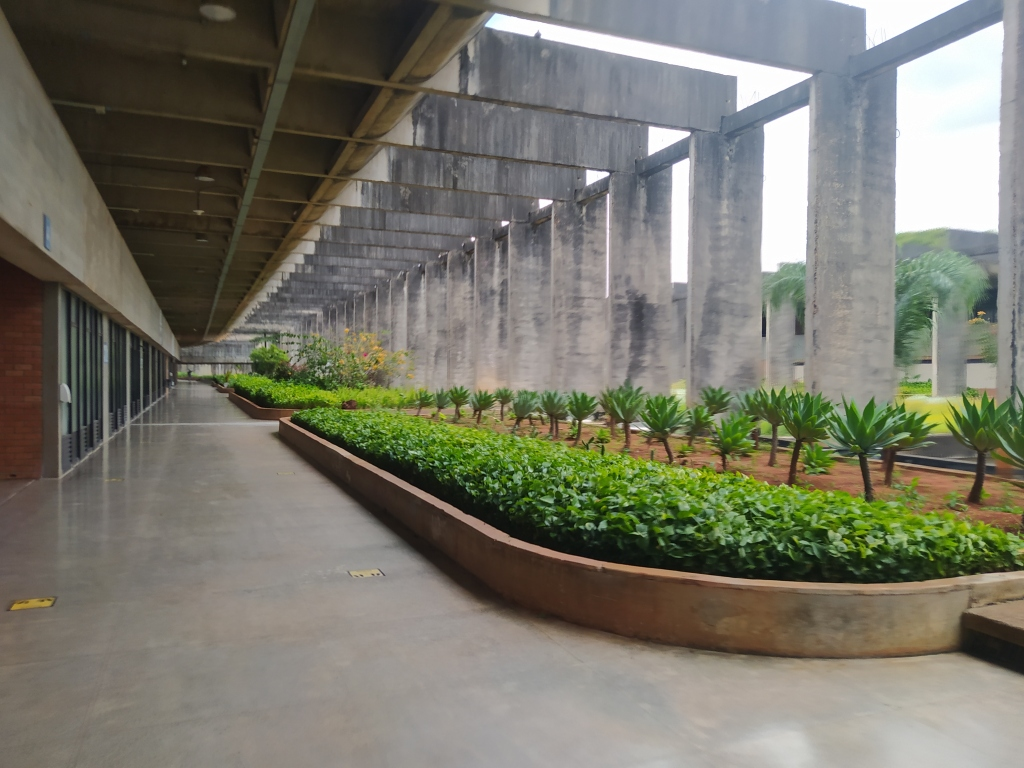
\includegraphics[width=\paperwidth]{images/unb.jpeg}}%
  % \setbeamercolor{normal text}{fg=black}
  % \setbeamercolor{frametitle}{fg=green}
  \maketitle
}

%-=-=-=-=-=-=-=-=-=-=-=-=-=-=-=-=-=-=-=-=-=-=-=-=
%	FRAME: Theme Package Requirements
%-=-=-=-=-=-=-=-=-=-=-=-=-=-=-=-=-=-=-=-=-=-=-=-=
\begingroup


%-=-=-=-=-=-=-=-=-=-=-=-=-=-=-=-=-=-=-=-=-=-=-=-=
%
%	TABLE OF CONTENTS: OVERVIEW
%
%-=-=-=-=-=-=-=-=-=-=-=-=-=-=-=-=-=-=-=-=-=-=-=-=

% {
% \usebackgroundtemplate{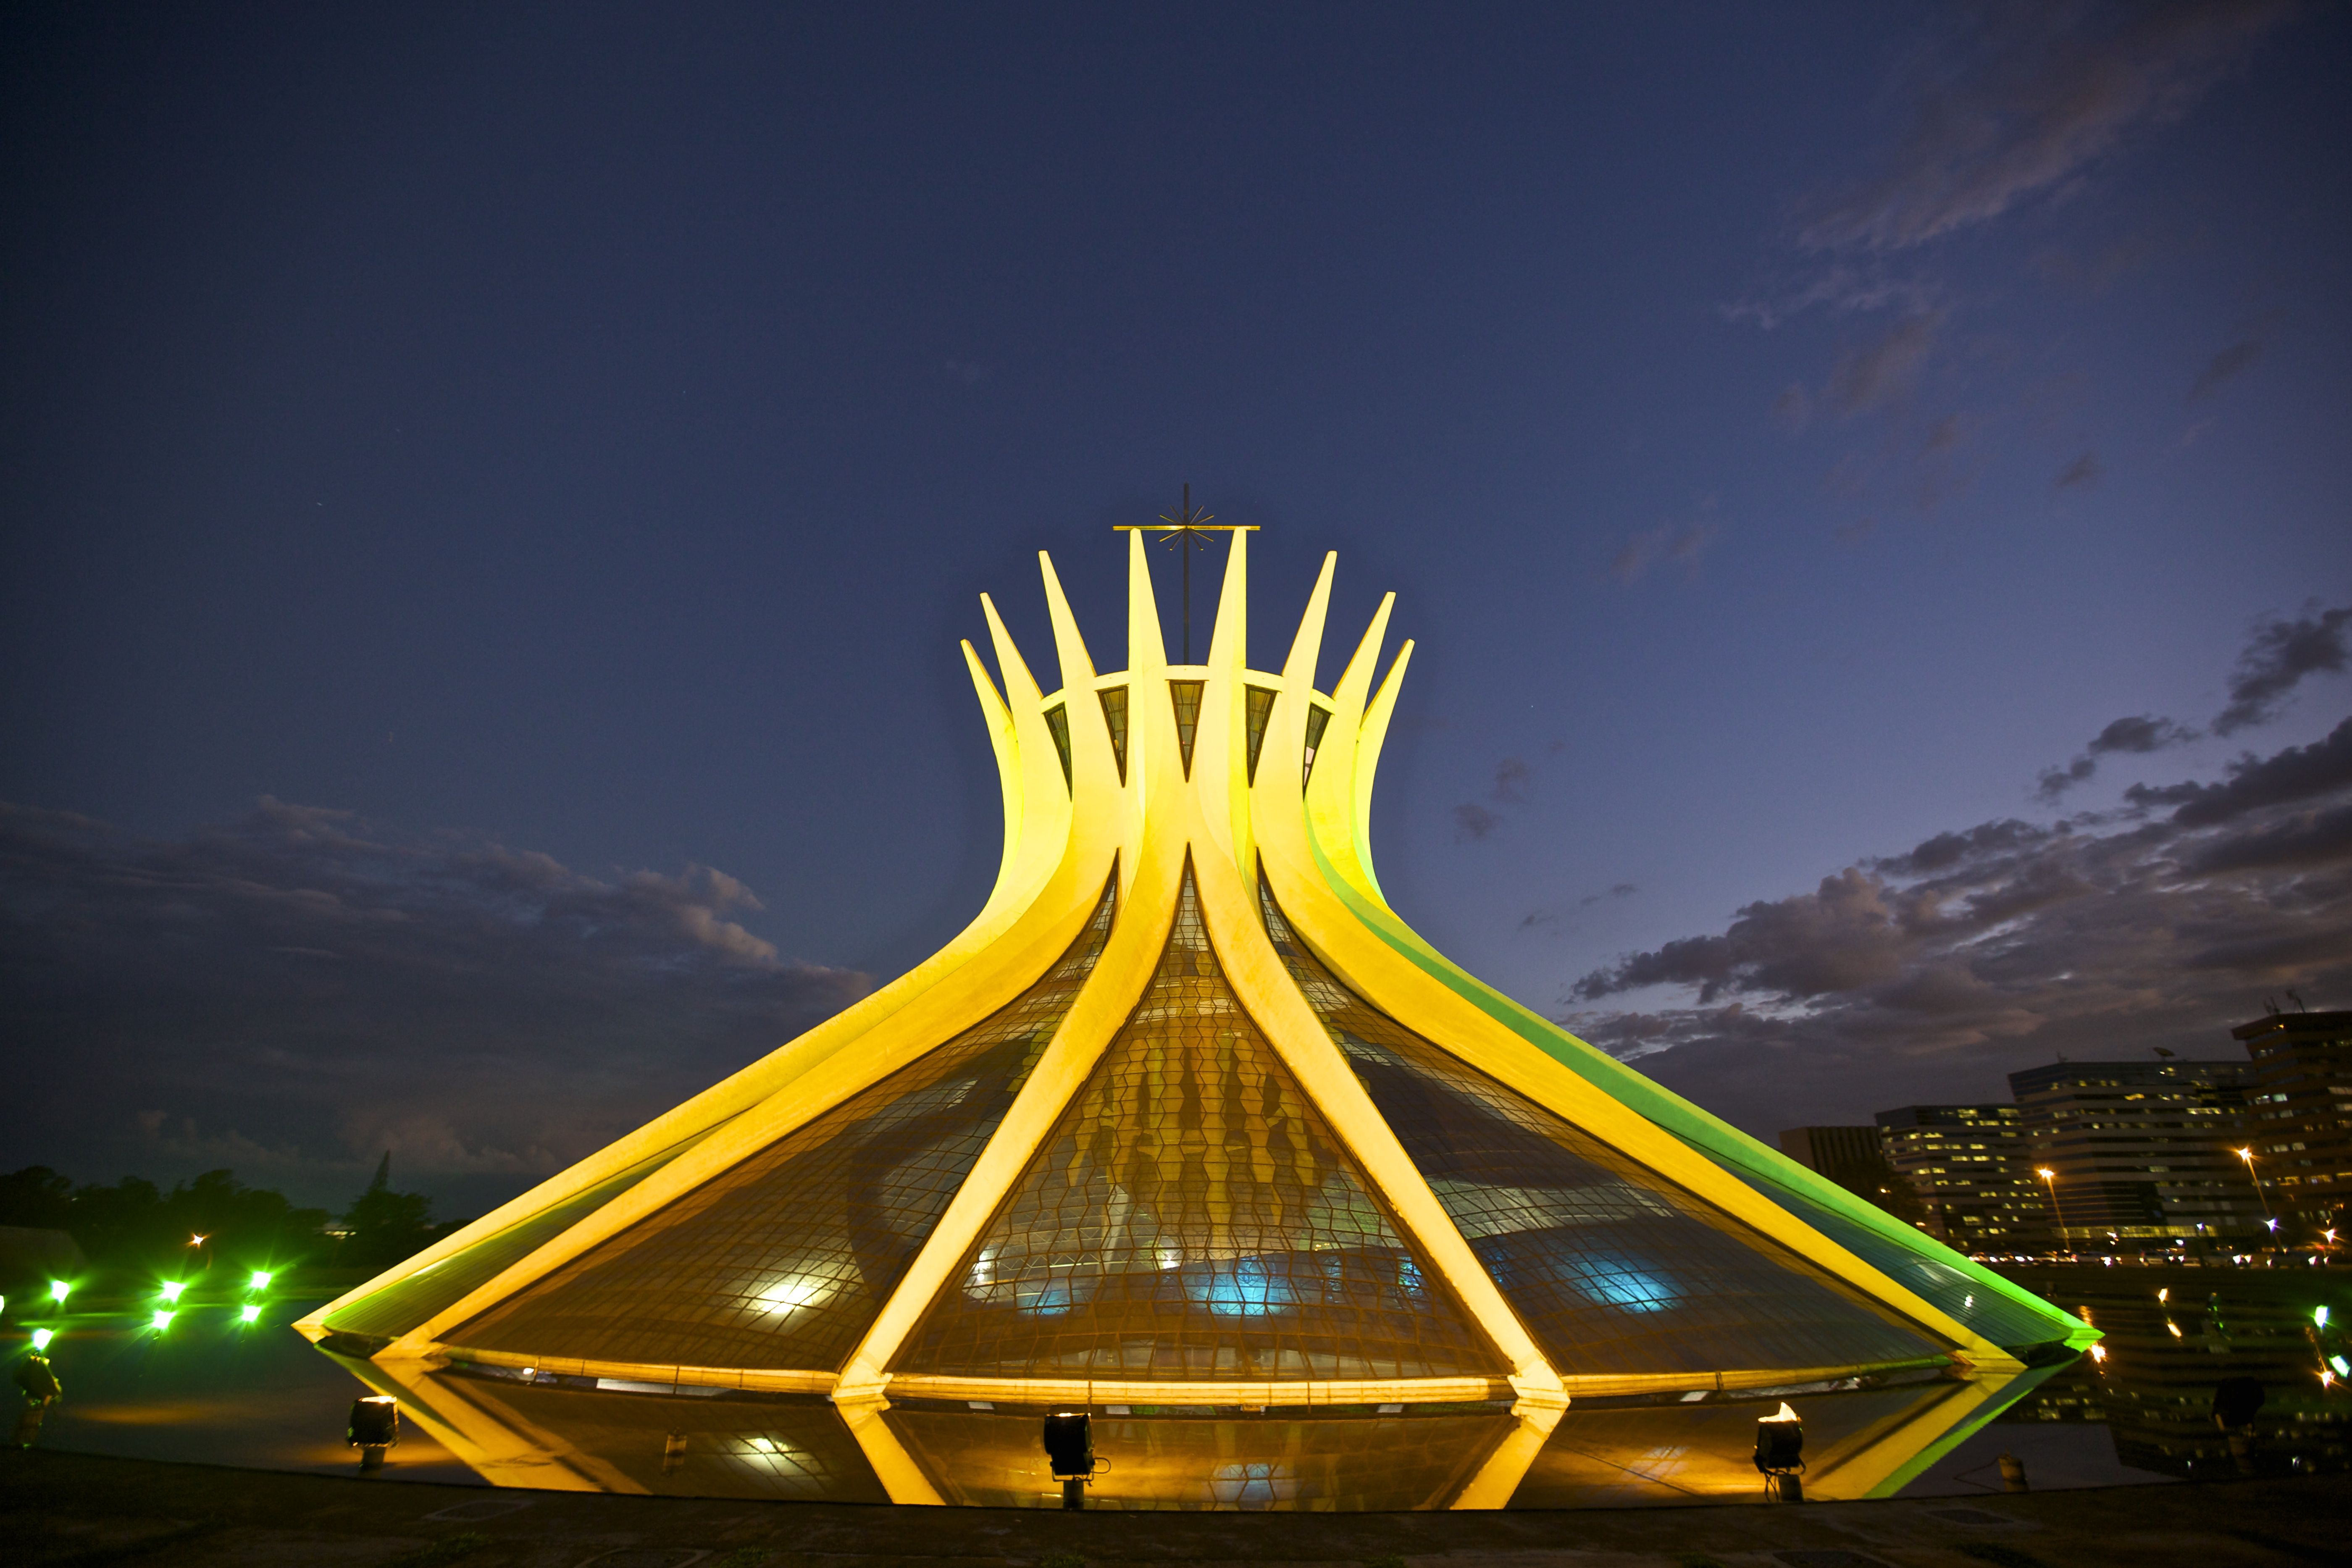
\includegraphics[width=\paperwidth]{images/brasilia1.jpg}}%
\section*{Overview}
\begin{frame}{{\color{white}Overview}}
% For longer presentations use hideallsubsections option
\tableofcontents[hideallsubsections]
\end{frame}
% }
%-=-=-=-=-=-=-=-=-=-=-=-=-=-=-=-=-=-=-=-=-=-=-=-=
%
%	TABLE OF CONTENTS: OVERVIEW
%
%-=-=-=-=-=-=-=-=-=-=-=-=-=-=-=-=-=-=-=-=-=-=-=-=

\section{General Information}

%-=-=-=-=-=-=-=-=-=-=-=-=-=-=-=-=-=-=-=-=-=-=-=-=
%	FRAME:
%-=-=-=-=-=-=-=-=-=-=-=-=-=-=-=-=-=-=-=-=-=-=-=-=

{
\usebackgroundtemplate{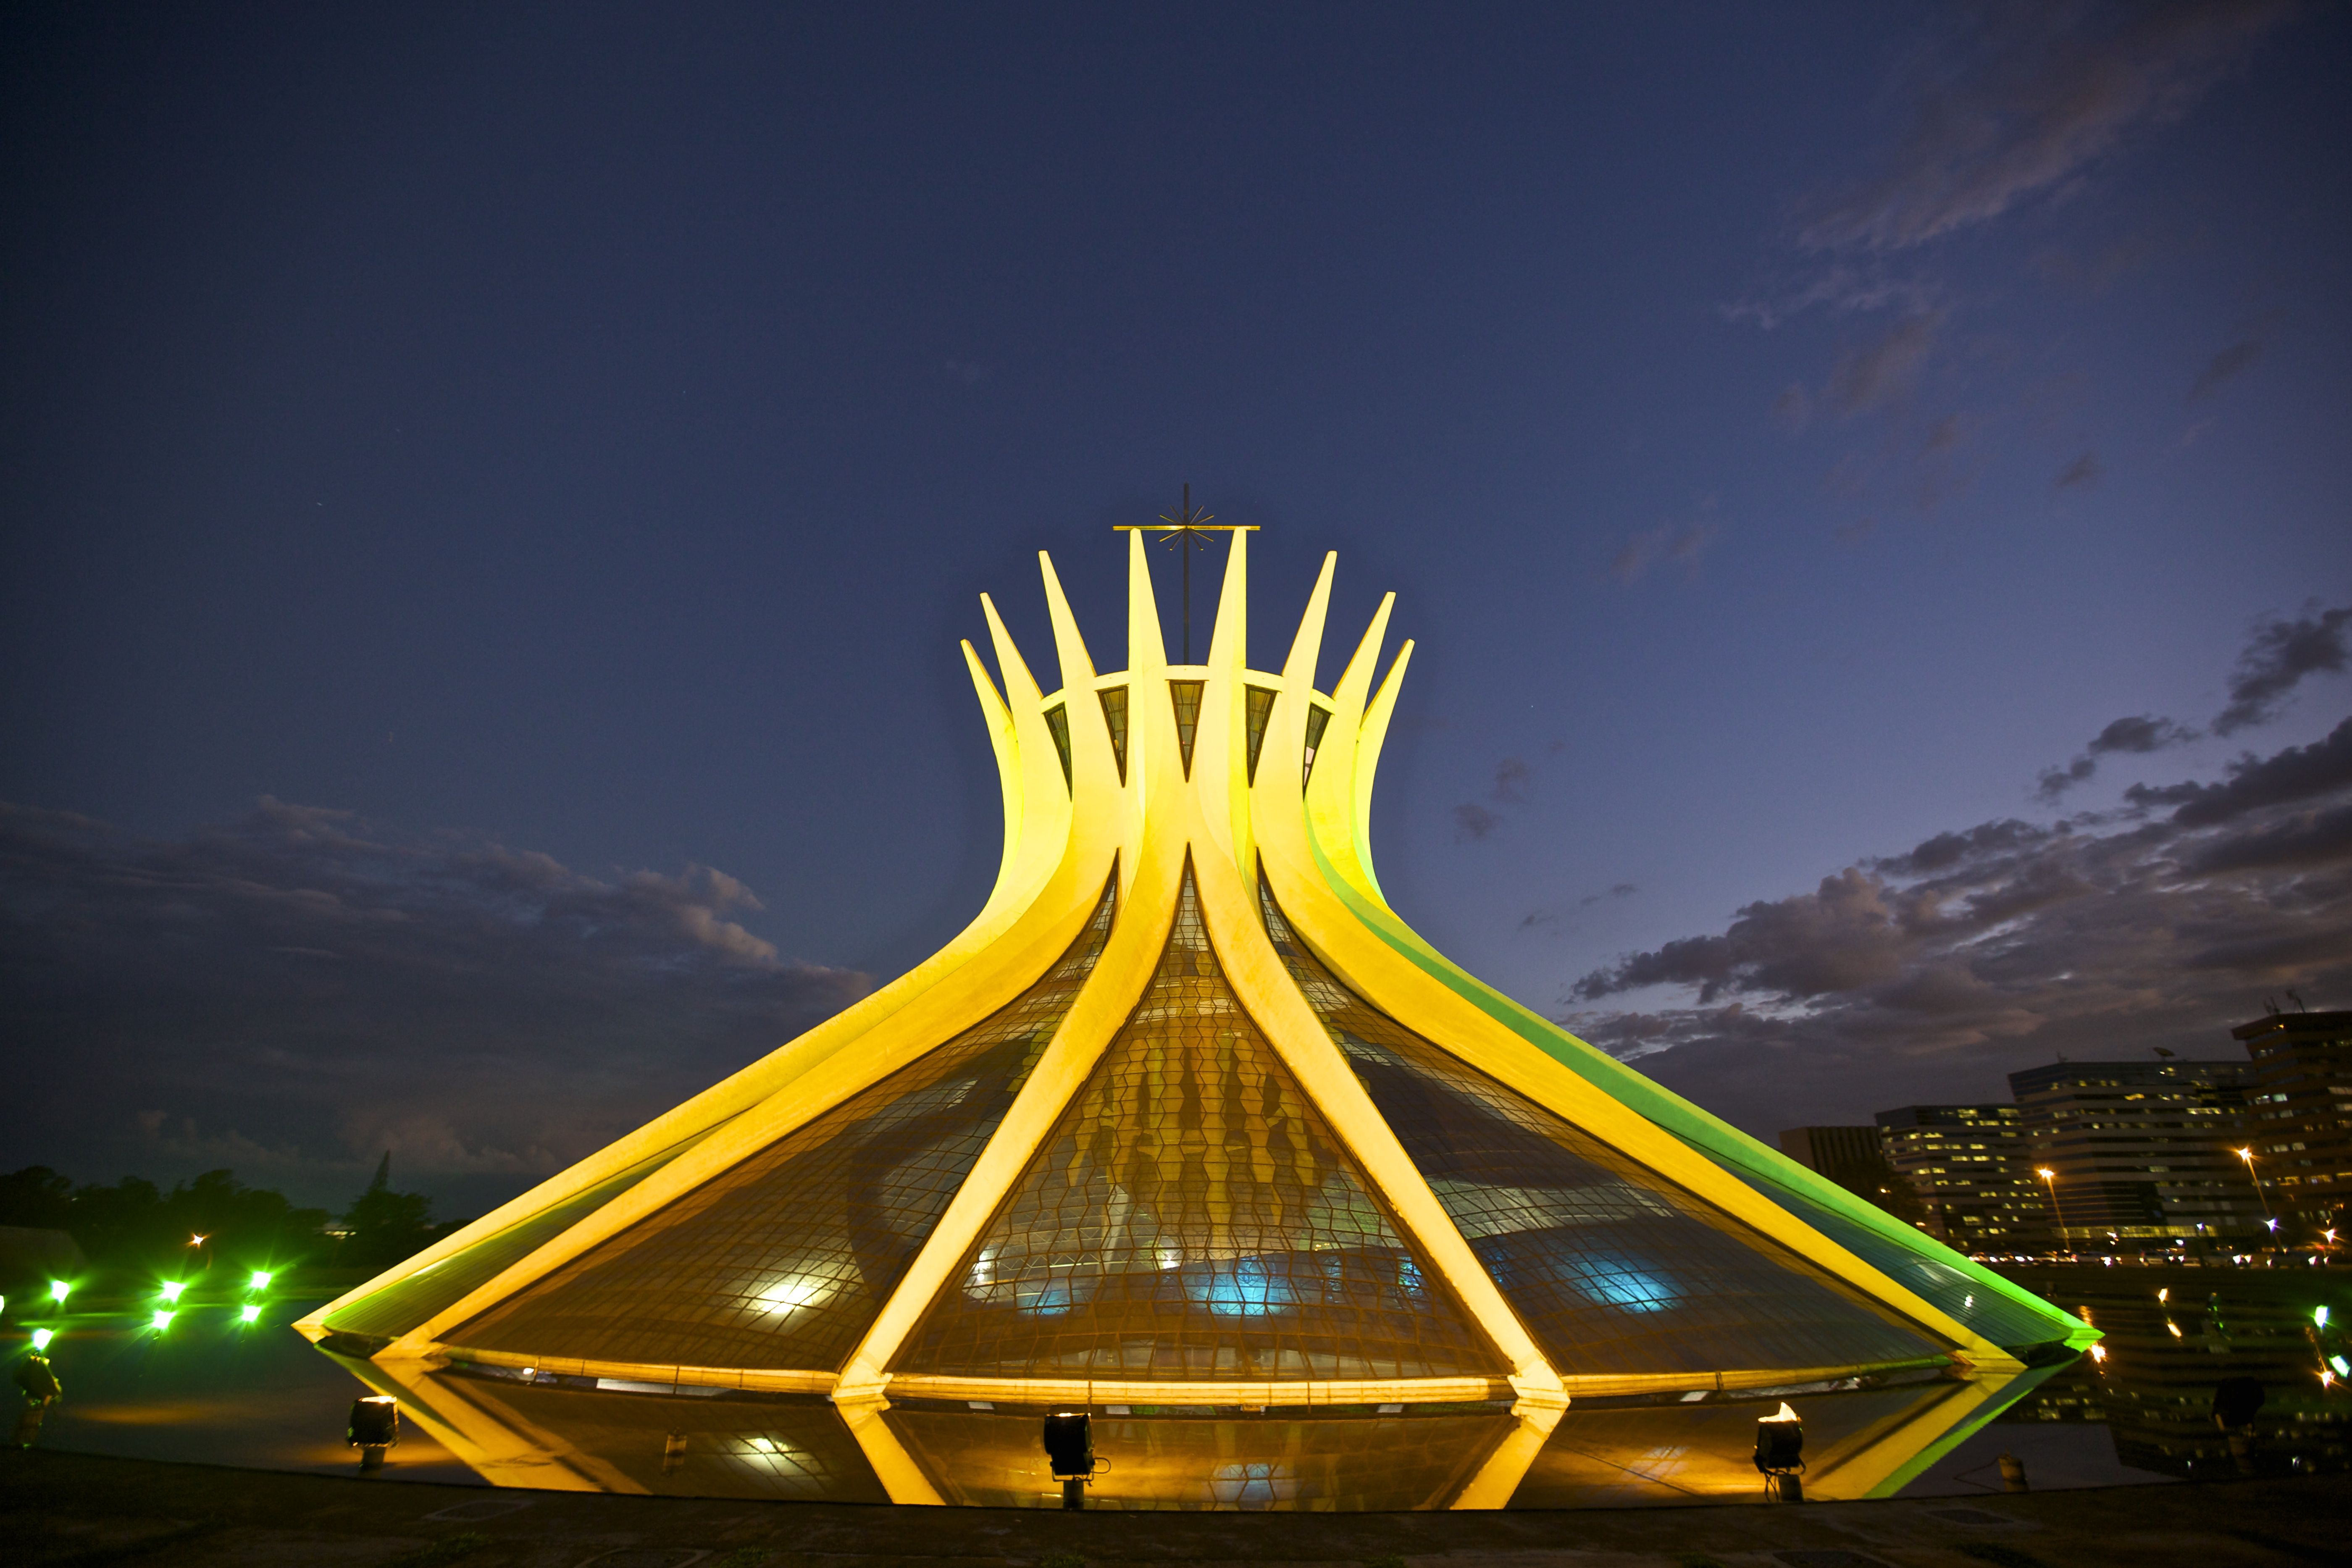
\includegraphics[width=\paperwidth]{images/brasilia1.jpg}}%
\setbeamercolor{itemize item}{fg=red}
\setbeamercolor{itemize subitem}{fg=blue}
\setbeamercolor{itemize subsubitem}{fg=cyan}
\setbeamertemplate{itemize item}[square]
\setbeamertemplate{itemize subitem}[circle]
\setbeamertemplate{itemize subsubitem}[triangle]
\begin{frame}[c]{Self-presentation (Who I am?)}

\begin{mybox}
\begin{itemize}
	\item {\color{white} A PhD student of Computer Science (since 2019)}
	\begin{itemize}
		\item {\color{white} Software Engineering Department (LES).}
            \item {\color{white} University of Brasilia (Capital of Brazil).}
            \item {\color{white} Department of software engineering (LES).}
            \begin{itemize}
		      \item {\color{white} The seventh best federal institution of Brazil (According to Times Higher Education World University Rankings 2023).}
                \item {\color{white} More than $39699$ undergraduate students.}
                \item {\color{white} More than $8819$ postgraduate students.}
	    \end{itemize}
	\end{itemize}
\end{itemize}
\end{mybox}

\end{frame}
}

%-=-=-=-=-=-=-=-=-=-=-=-=-=-=-=-=-=-=-=-=-=-=-=-=
%	FRAME:
%-=-=-=-=-=-=-=-=-=-=-=-=-=-=-=-=-=-=-=-=-=-=-=-=

\begin{frame}{It is Brasília!}

\begin{columns}[t]
\column{.5\textwidth}
\centering
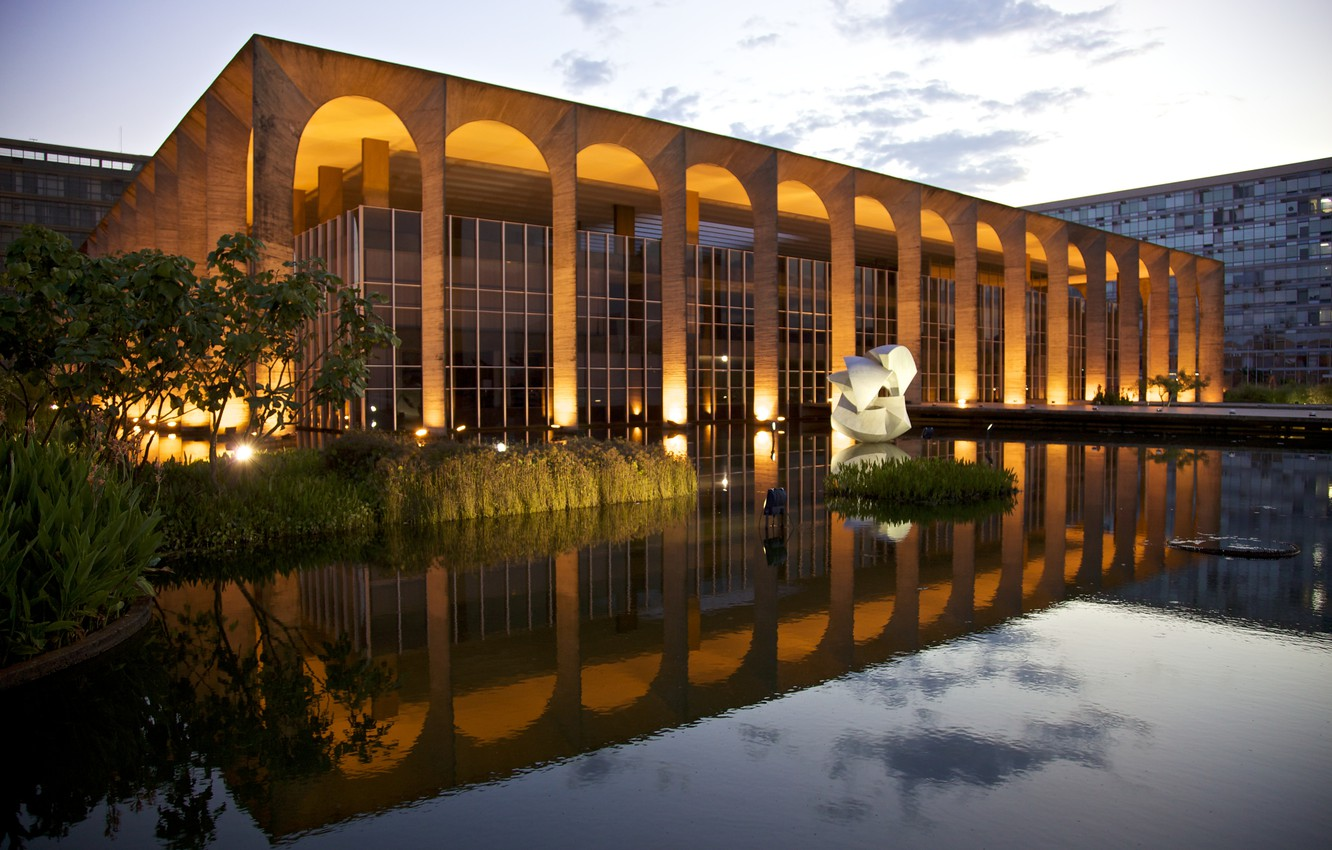
\includegraphics[width=6cm,height=3.8cm]{images/itamaraty-palace-braslia.jpg}\\
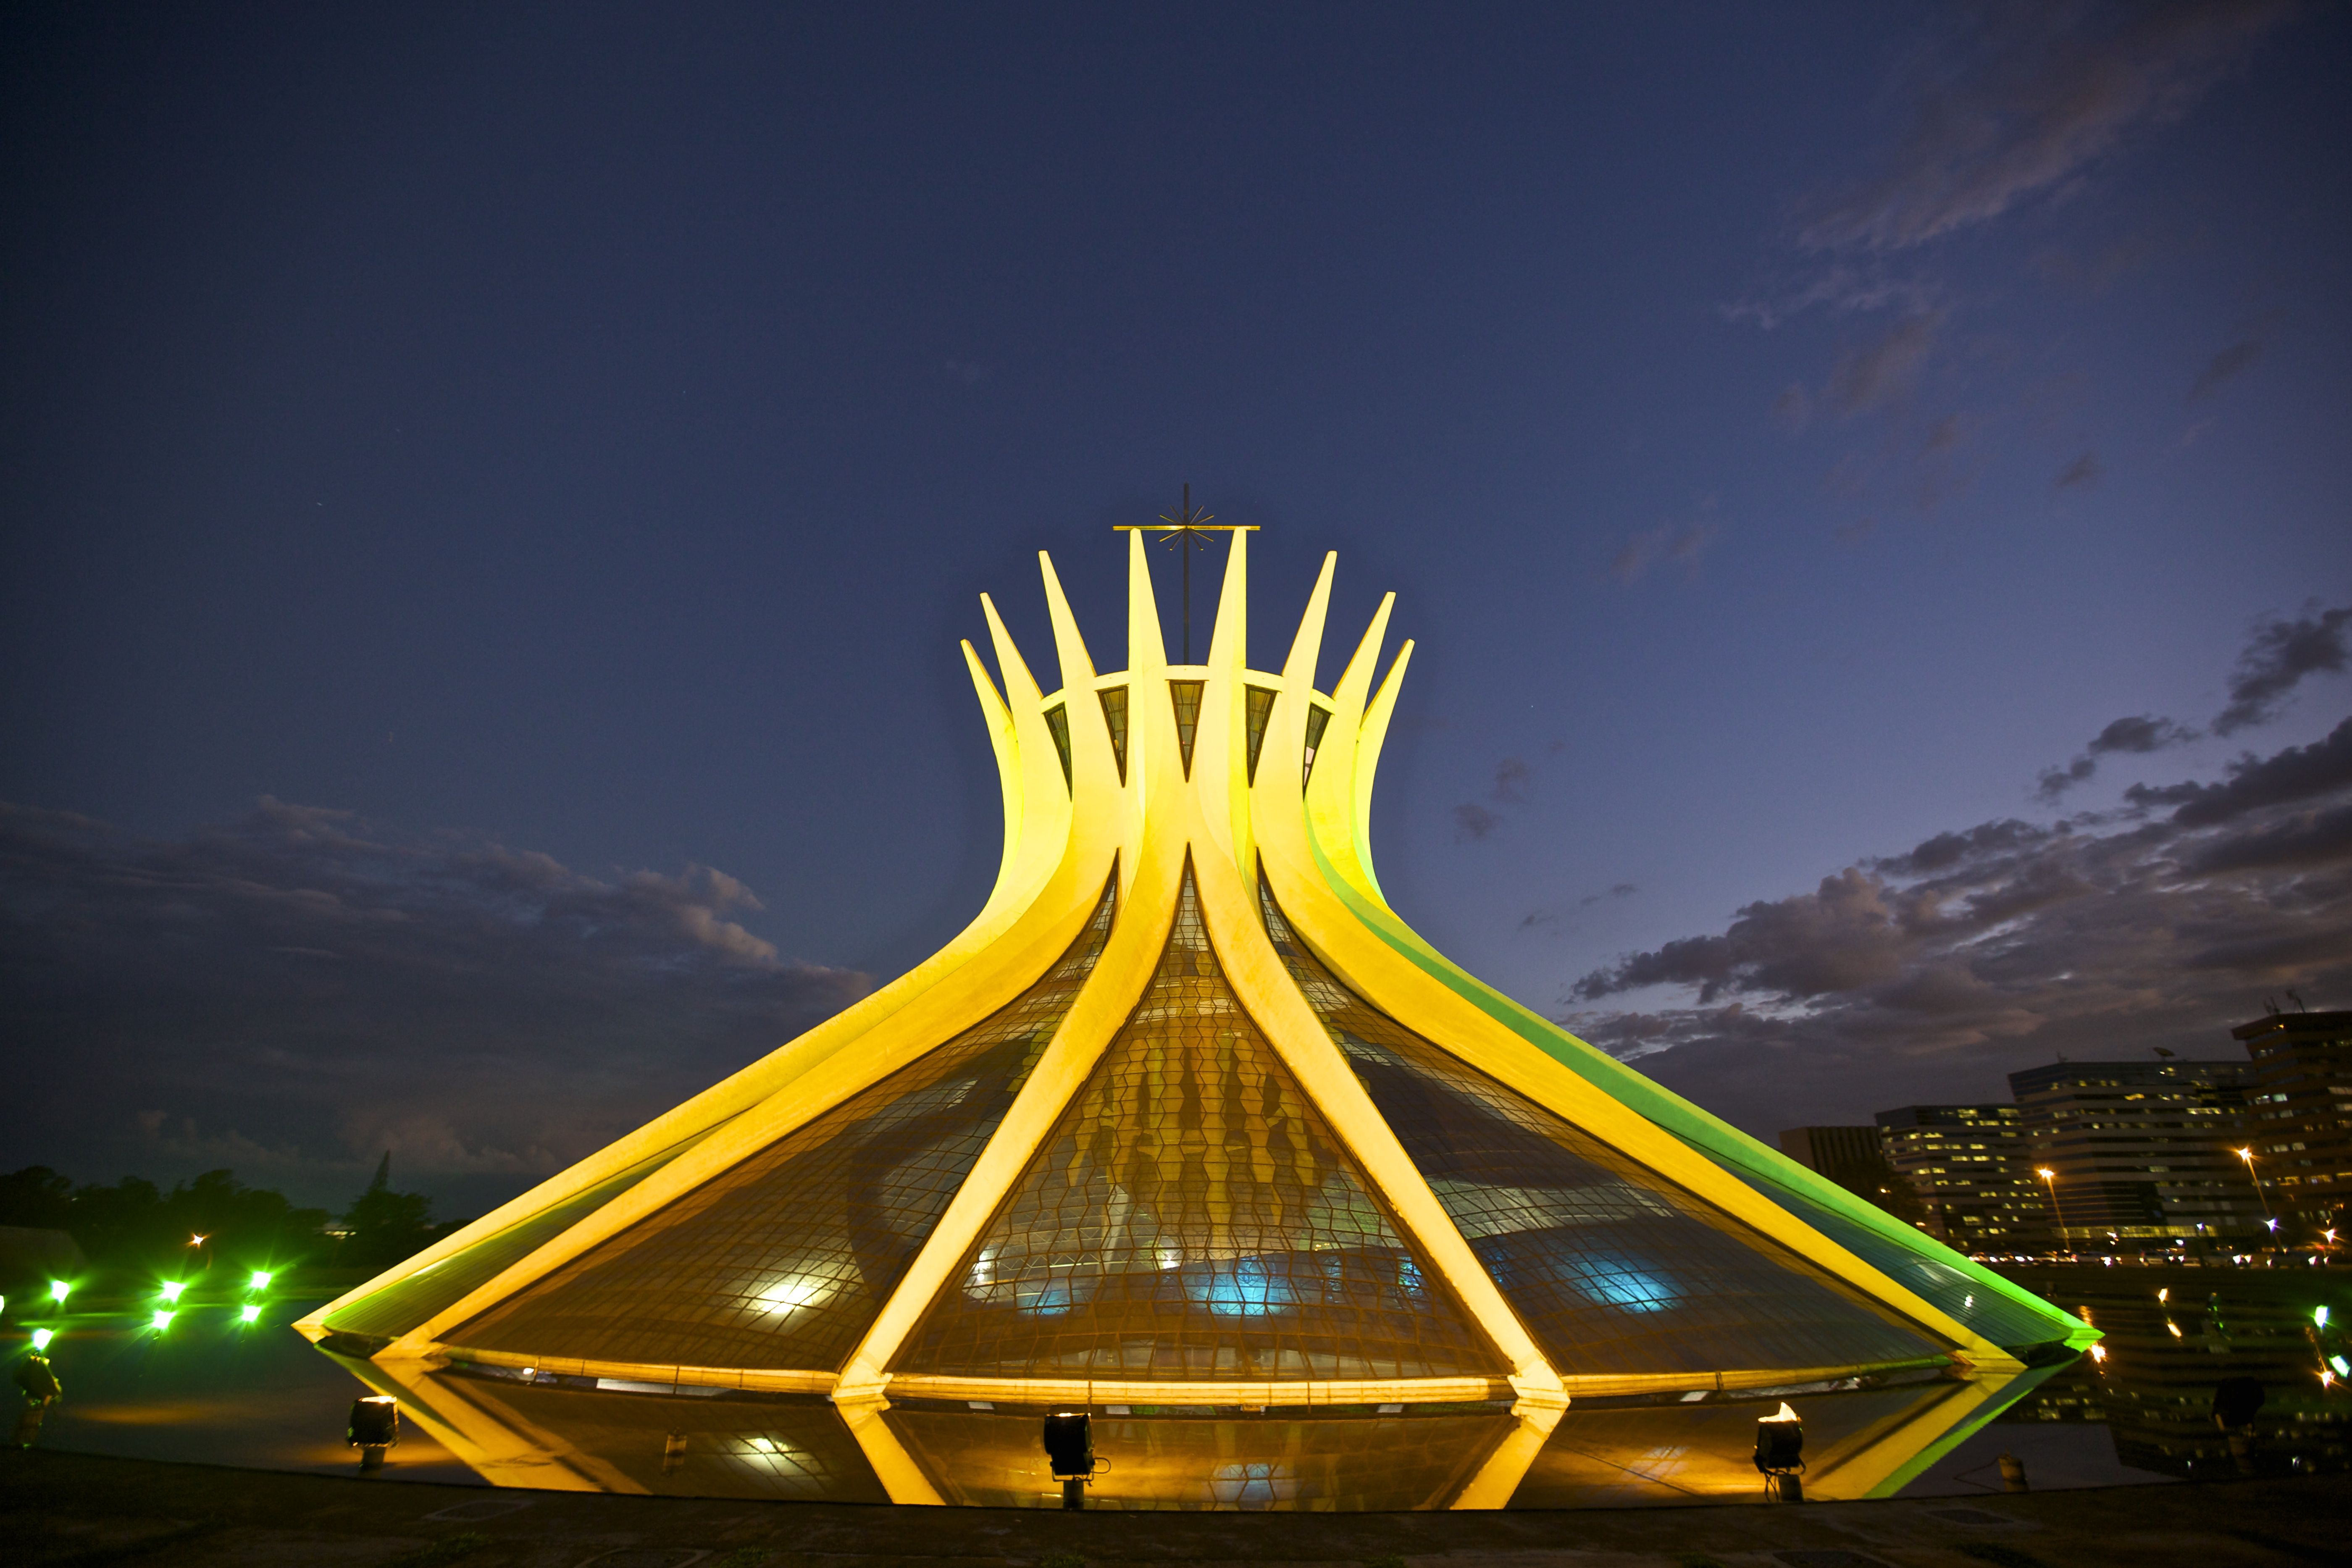
\includegraphics[width=6cm,height=3.8cm]{images/brasilia1.jpg}
\column{.5\textwidth}
\centering
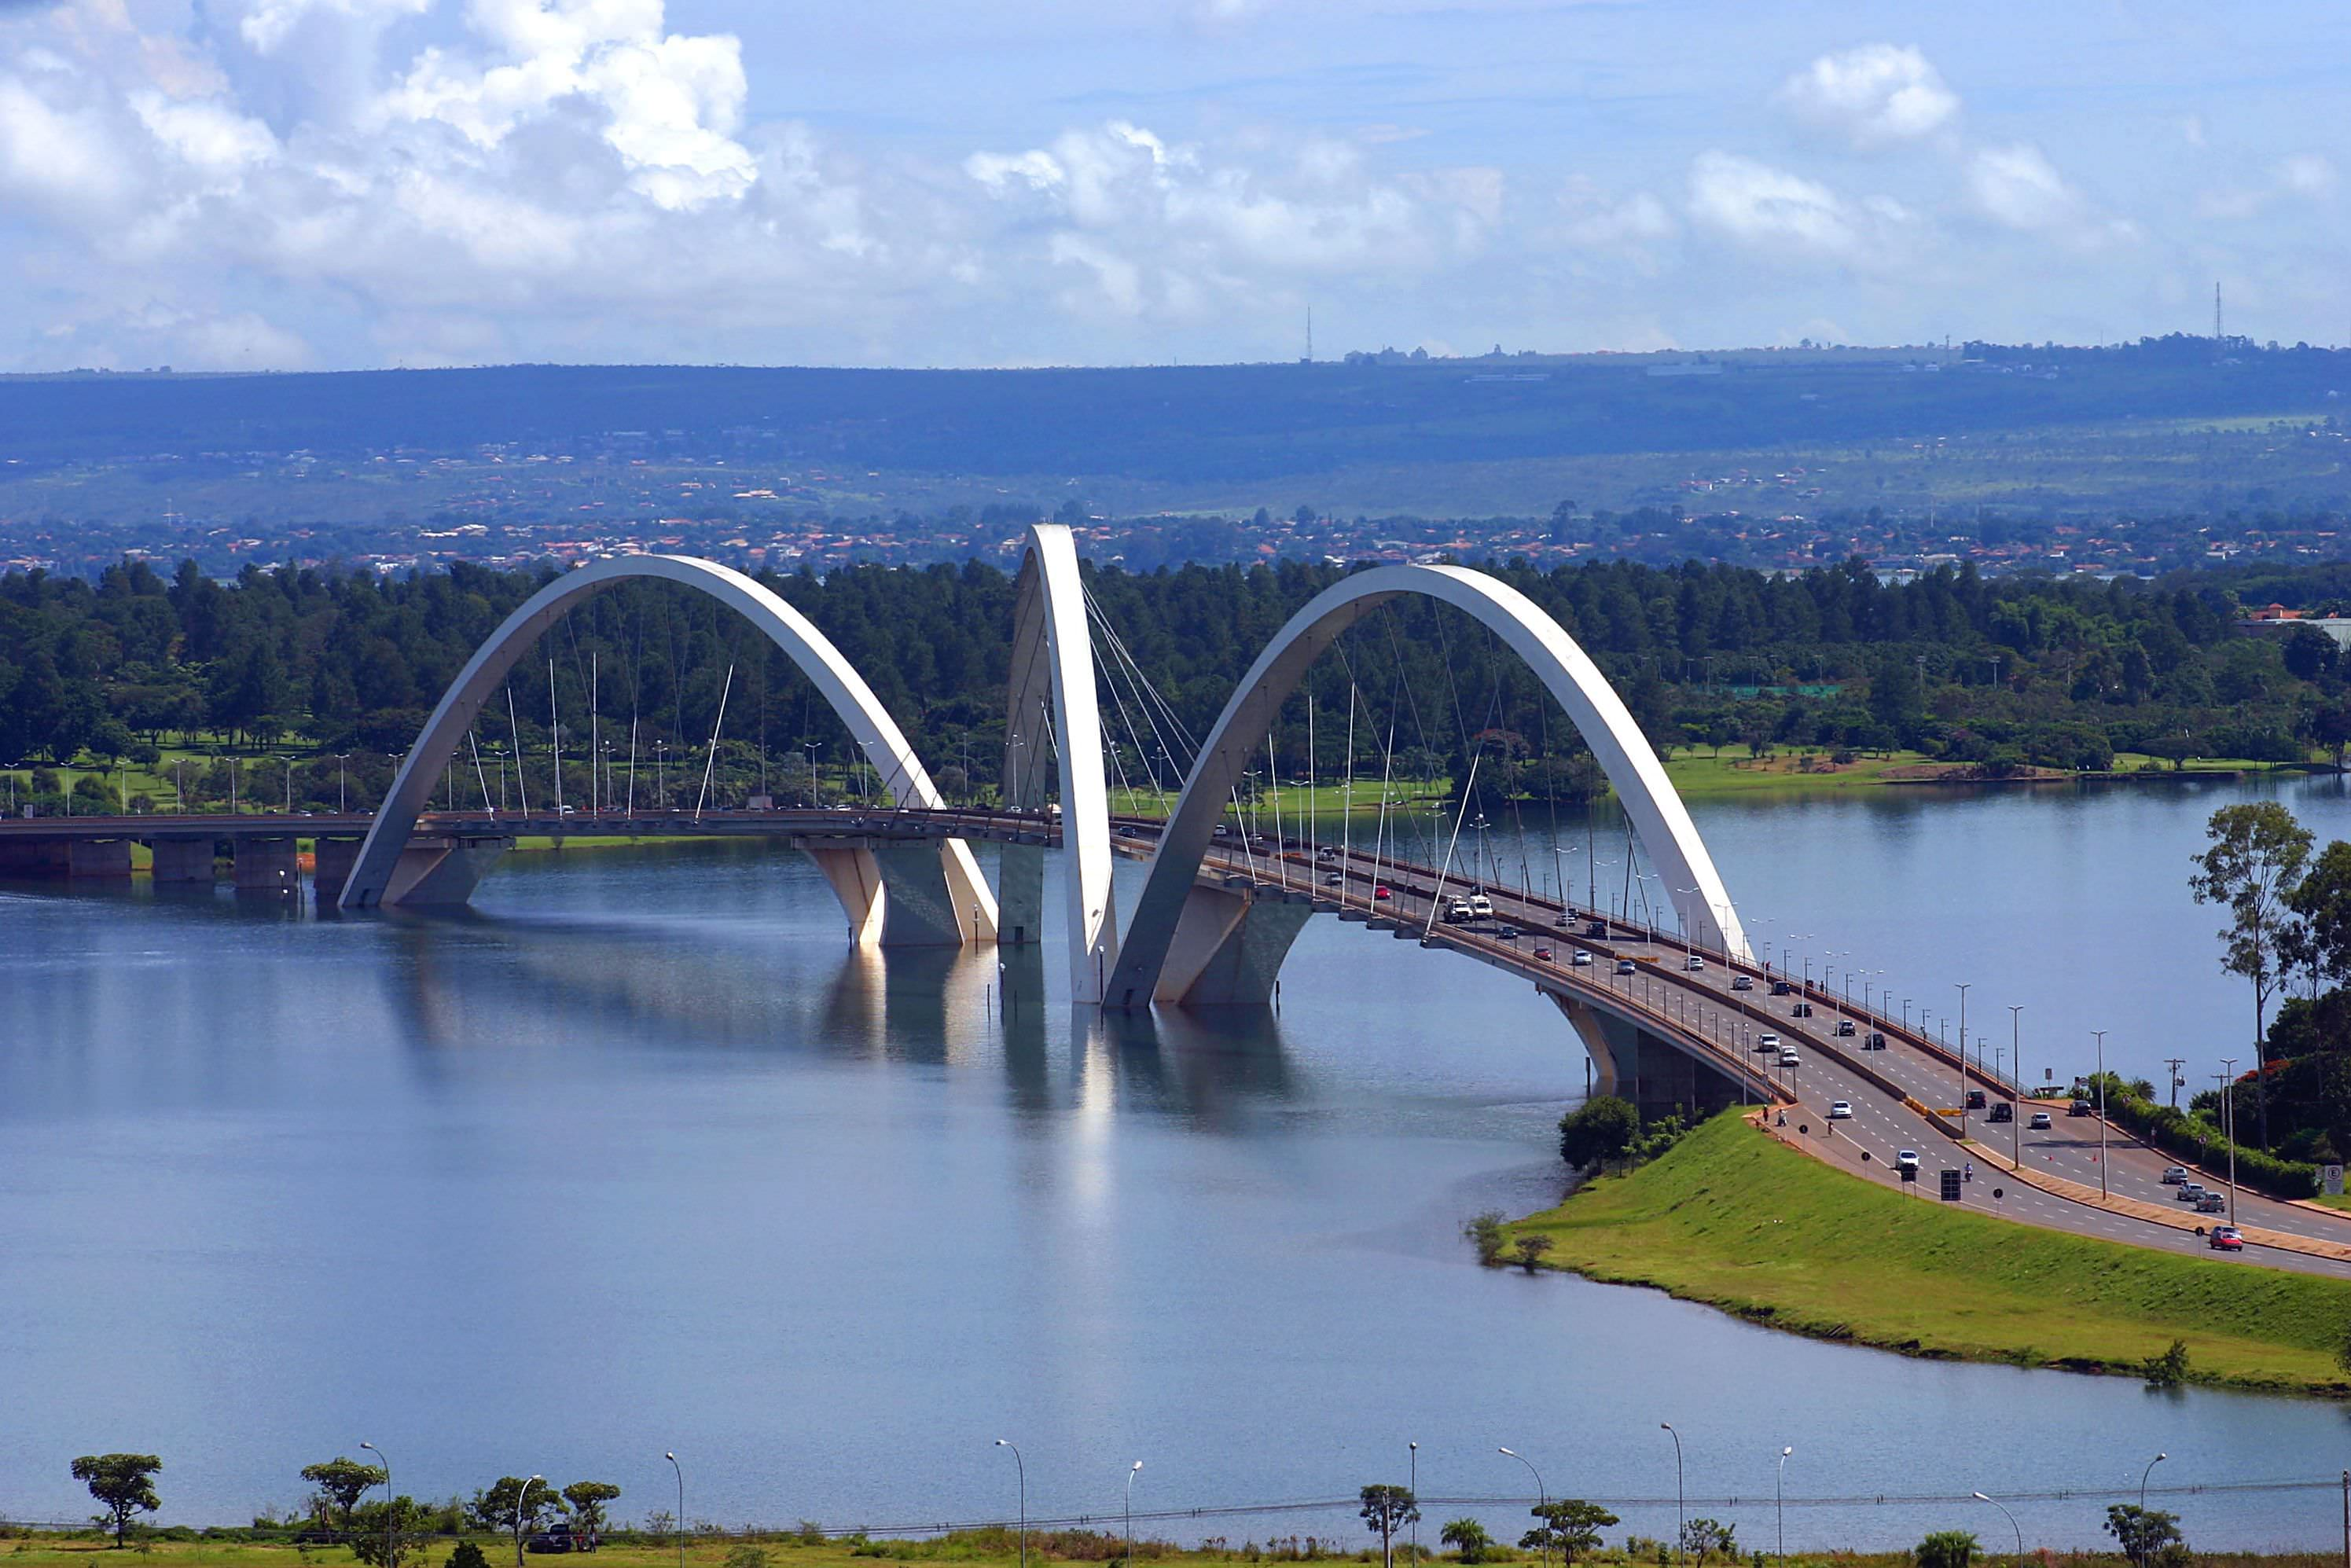
\includegraphics[width=6cm,height=3.8cm]{images/bridge-bsb.jpg}\\
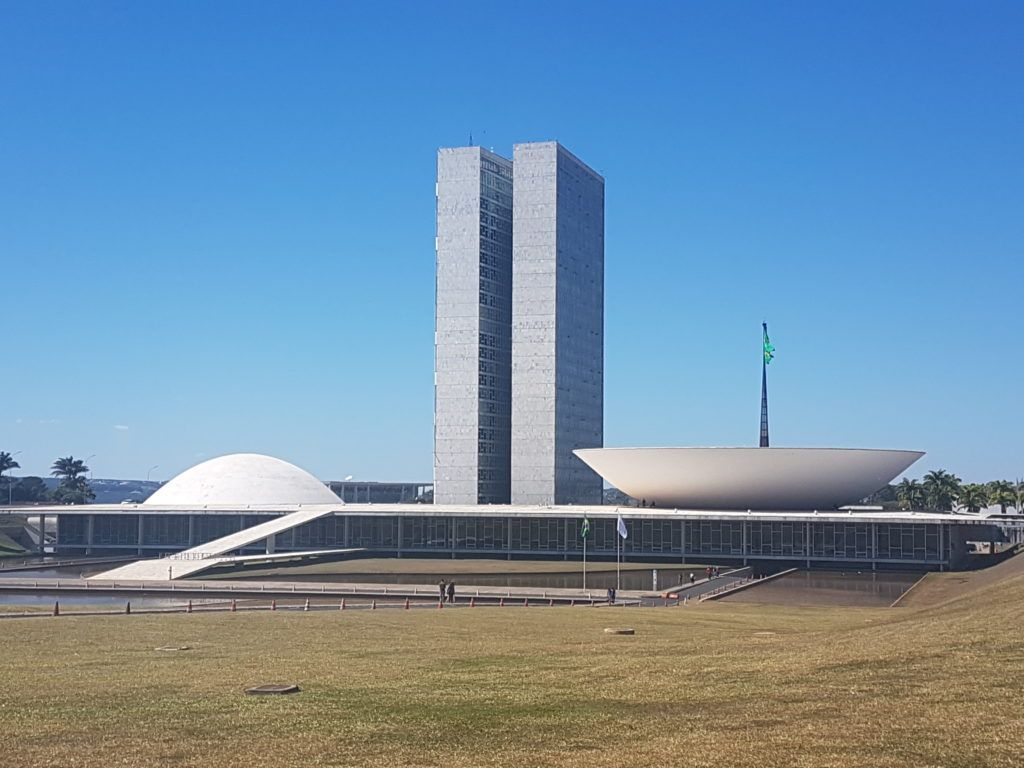
\includegraphics[width=6cm,height=3.8cm]{images/praca-poderes.jpg}
\end{columns}
    
\end{frame}



\begin{frame}[c]{International Visiting Researcher Programme}
	
% \alert{sthlm} continues to be a theme that can easily be modified through the style files.  If you are looking for a packaged theme, then I highly recommend \alert{mTheme}.\\

% \vspace{1em}

% I use a custom version of \alert{sthlm} for daily decks and make a vanilla version of the theme available for others to use and modify. - Enjoy!

\begin{figure}
    \centering
    \caption{The publication of the visiting researchers that is done by the INESC TEC magazine.}
    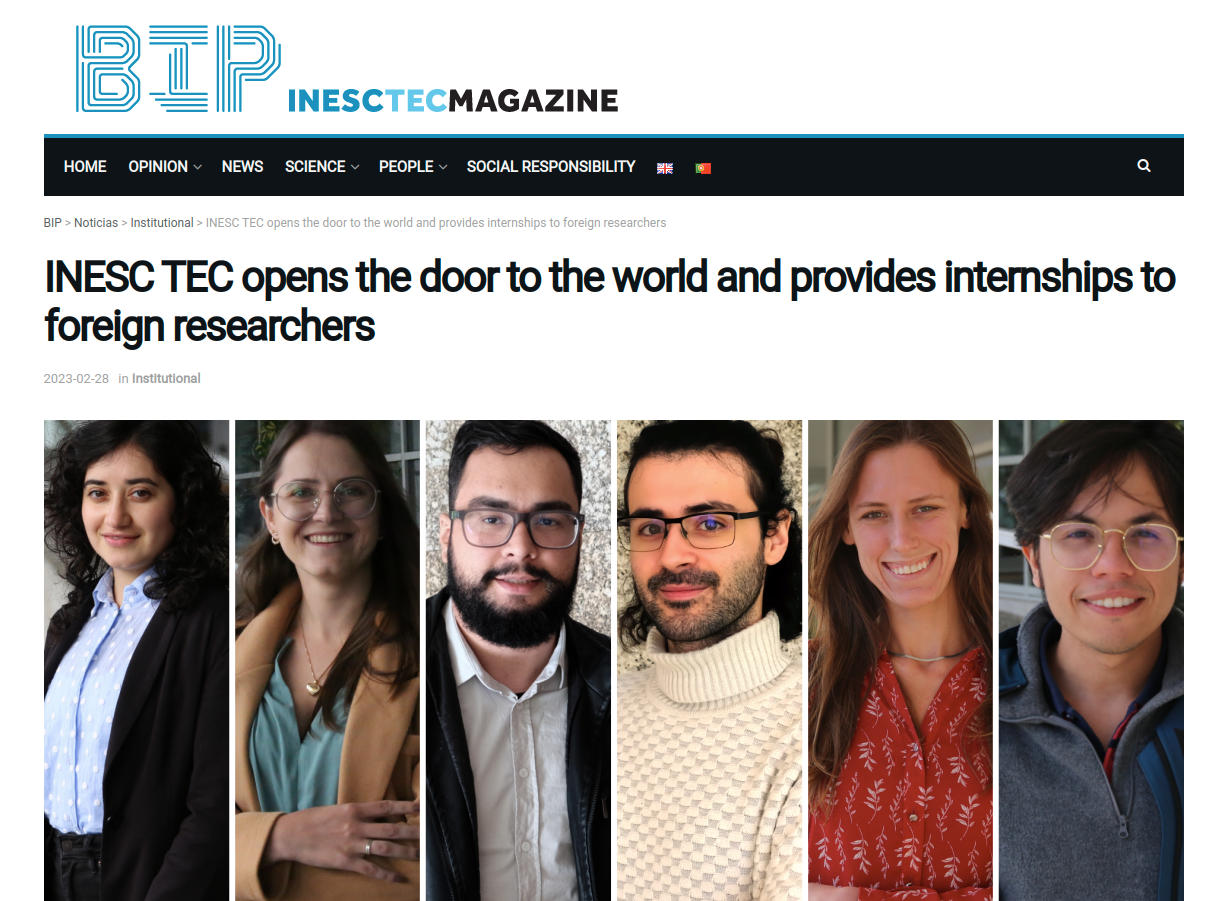
\includegraphics[width=\textwidth]{images/bip-inesctec-pt.png}
    \label{fig:my_label}
\end{figure}

\end{frame}



\section{Motivations, Questions and Problems of Research}

{
\usebackgroundtemplate{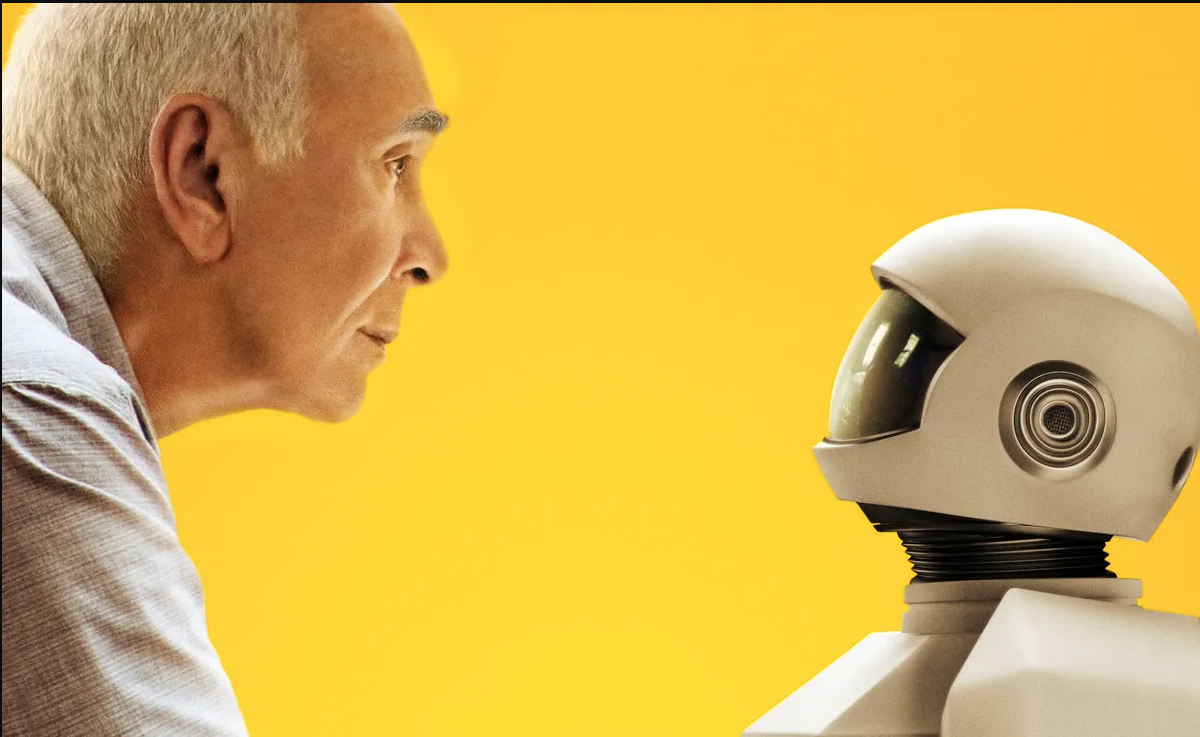
\includegraphics[width=\paperwidth,height=\paperheight]{images/aging.png}}%
\begin{frame}[c]{Introduction and Motivation}

\centering
Software aging \\
{\centering David Parnas (1994)}

% \begin{figure}
%     \centering
%     \includegraphics[width=\textwidth]{}
%     \caption{Caption}
%     \label{fig:my_label}
% \end{figure}
% \cRed{sthlm} theme has been designed and tested to work within the SageMathCloud (Linux) environment.\\

% \vspace{1em}

% \begin{alertblock}{Warning of Build Issues}
% \color{white} I cannot guarantee that the code used to create the sthlm theme is \emph{error free}, \emph{optimized}, \emph{well written} nor \emph{if it will work in your production environment}.
% \end{alertblock}

\end{frame}
}

%-=-=-=-=-=-=-=-=-=-=-=-=-=-=-=-=-=-=-=-=-=-=-=-=
%	FRAME:
%-=-=-=-=-=-=-=-=-=-=-=-=-=-=-=-=-=-=-=-=-=-=-=-=

\begin{frame}[c]{What can I do to delay a aging of software?}

    {\footnotesize According to Bragagnolo et al.~\footnote{\emph{\footnotesize Bragagnolo, Santiago, et al. Software migration: A theoretical framework (a grounded theory approach on systematic literature review) - 2021.}}, we can conduct some software migration approaches, such as:}
{\scriptsize
   \begin{itemize}
        % This involves moving the codebase of an application from one platform or language to another. 
        \item \textbf{Language migration}: For example, migrating from a legacy programming language like COBOL to a modern language like Java.
        % This involves transferring data from one database to another, usually for the purpose of upgrading to a newer or more powerful database management system.
        \item \textbf{Database migration}: For example, migrating from MySQL to PostgreSQL.

        % This involves moving an application from one operating system or hardware platform to another.
        \item \textbf{Platform migration}:  For example, migrating from a Unix-based platform to a Windows-based platform.
        % This involves changing the underlying architecture of an application, usually to improve its scalability or performance.
        \item \textbf{Architecture migration}:  For example, migrating from a monolithic architecture to a microservices architecture.
        % This involves migrating an application from one software framework to another.
        \item \textbf{Framework migration}: For example, migrating a web application from the JSF (Java Server Faces) framework to the Spring framework.
        % This involves moving an application from on-premises servers to cloud-based servers or from one cloud provider to another.
        \item \textbf{Cloud migration}: For example, migrating a web application from a self-hosted server to AWS.
   \end{itemize}
}
% \emph{\small PIRKELBAUER, Peter; DECHEV, Damian; STROUSTRUP, Bjarne - Source code rejuvenation is not refactoring. (SOFSEM 2010)}
\end{frame}


%-=-=-=-=-=-=-=-=-=-=-=-=-=-=-=-=-=-=-=-=-=-=-=-=
%	FRAME:
%-=-=-=-=-=-=-=-=-=-=-=-=-=-=-=-=-=-=-=-=-=-=-=-=

\begin{frame}[c]{Source code rejuvenation approach}


According to PIRKELBAUER et al.~\footnote{\emph{PIRKELBAUER, Peter; DECHEV, Damian; STROUSTRUP, Bjarne - Source code rejuvenation is not refactoring. (SOFSEM 2010)}}, source code rejuvenation may be interpreted as the replacement of legacy functionality with newer ones offered by new versions of the programming language.

\end{frame}

\begin{frame}[c]{A Simple System Model}

\begin{figure}
    \centering
    \caption{\footnotesize UML diagram to illustrate the model adapted from 101companies~\footnote{\tiny Favre, Jean-Marie, et al. \emph{101companies: a community project on software technologies and software languages." Objects, Models, Components, Patterns} - (TOOLS 2012)}}
    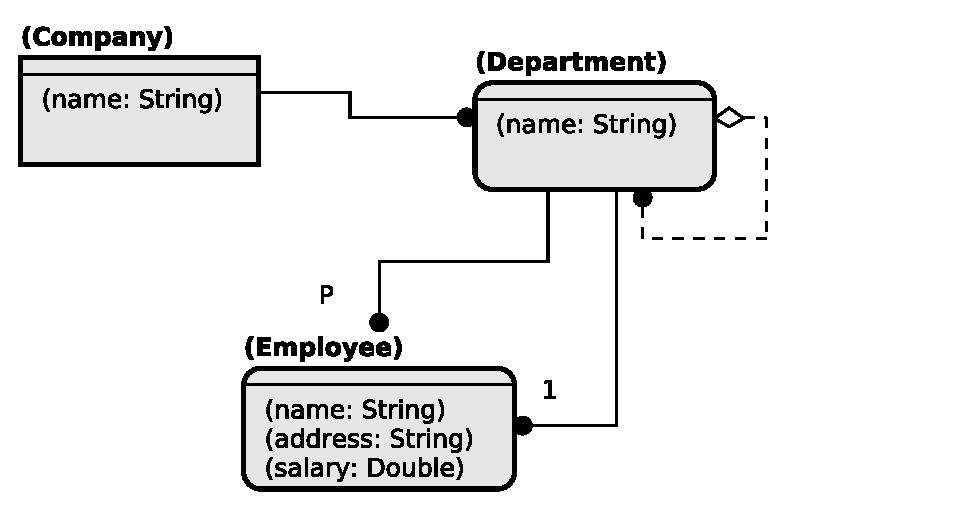
\includegraphics[width=\textwidth]{images/er-companies.pdf}
    \label{fig:101companies}
\end{figure}

\end{frame}

%-=-=-=-=-=-=-=-=-=-=-=-=-=-=-=-=-=-=-=-=-=-=-=-=
%	FRAME:
%-=-=-=-=-=-=-=-=-=-=-=-=-=-=-=-=-=-=-=-=-=-=-=-=

\defverbatim[colored]\lstI{
\begin{lstlisting}[language=C++,basicstyle=\tiny,keywordstyle=\color{red},tabsize=2,showspaces=false,showstringspaces=false,caption={Implementation following a traditional $for \; loop$ approach.},captionpos=t]
class Department {
[...]
 void cutEmployeeSalaries(double percentage) {
     for (int i = 0; i < employees.size(); i++) {
         employees[i]->cutSalary(percentage);
     }
 }
[...]
\end{lstlisting}
}

\defverbatim[colored]\lstII{
\begin{lstlisting}[language=C++,basicstyle=\tiny,keywordstyle=\color{red},tabsize=2,showspaces=false,showstringspaces=false,caption={implementation using a $range-based \;for\; loop$ and $auto-typed \; variables$.},captionpos=t]
class Department {
[...]
 void cutEmployeeSalaries(double percentage) {
    for (auto emp : employees) {
        emp->cutSalary(percentage);
    }
 }
[...]
\end{lstlisting}
}

\begin{frame}[c]{Source code rejuvenation approach}{C++}

\lstI
\lstII

\end{frame}

%-=-=-=-=-=-=-=-=-=-=-=-=-=-=-=-=-=-=-=-=-=-=-=-=
%	FRAME:
%-=-=-=-=-=-=-=-=-=-=-=-=-=-=-=-=-=-=-=-=-=-=-=-=

\begin{frame}[c]{Research related to code rejuvenation}

\begin{itemize}
\item Reconciling the past and the present: An empirical study on the application of source code transformations to automatically rejuvenate Java programs - SANER (2018);
\item Does the Introduction of Lambda Expressions Improve the Comprehension of Java Programs? - SBES (2019)
\item Understanding the Impact of Introducing Lambda Expressions in Java Programs - JSERD (2020);
\end{itemize}


\end{frame}

%-=-=-=-=-=-=-=-=-=-=-=-=-=-=-=-=-=-=-=-=-=-=-=-=
%	FRAME:
%-=-=-=-=-=-=-=-=-=-=-=-=-=-=-=-=-=-=-=-=-=-=-=-=

\begin{frame}[c]{Research Questions}

\begin{block}{What are the motivations that lead software developers to rejuvenate their software?}
{\color{white} This question aims to understand what factors, phenomena, and situations lead developers to rejuvenate their codes.}
\end{block}

\begin{block}{What are the challenges that hinder software developers from rejuvenating their software?}
{\color{white} This question aims to explain which situations and factors make it difficult or prevent developers to rejuvenate their programs.}
\end{block}

\end{frame}

% %-=-=-=-=-=-=-=-=-=-=-=-=-=-=-=-=-=-=-=-=-=-=-=-=
% %	TEMPLATE OF BASIC FRAME
% %-=-=-=-=-=-=-=-=-=-=-=-=-=-=-=-=-=-=-=-=-=-=-=-=

% \begin{frame}[c]{Research Questions}

% \end{frame}

\section{Thesis Proposal}

%-=-=-=-=-=-=-=-=-=-=-=-=-=-=-=-=-=-=-=-=-=-=-=-=
%	FRAME:
%-=-=-=-=-=-=-=-=-=-=-=-=-=-=-=-=-=-=-=-=-=-=-=-=

\begin{frame}{Thesis Proposal}
\centering
\begin{figure}
        \caption{Thesis planing.}
	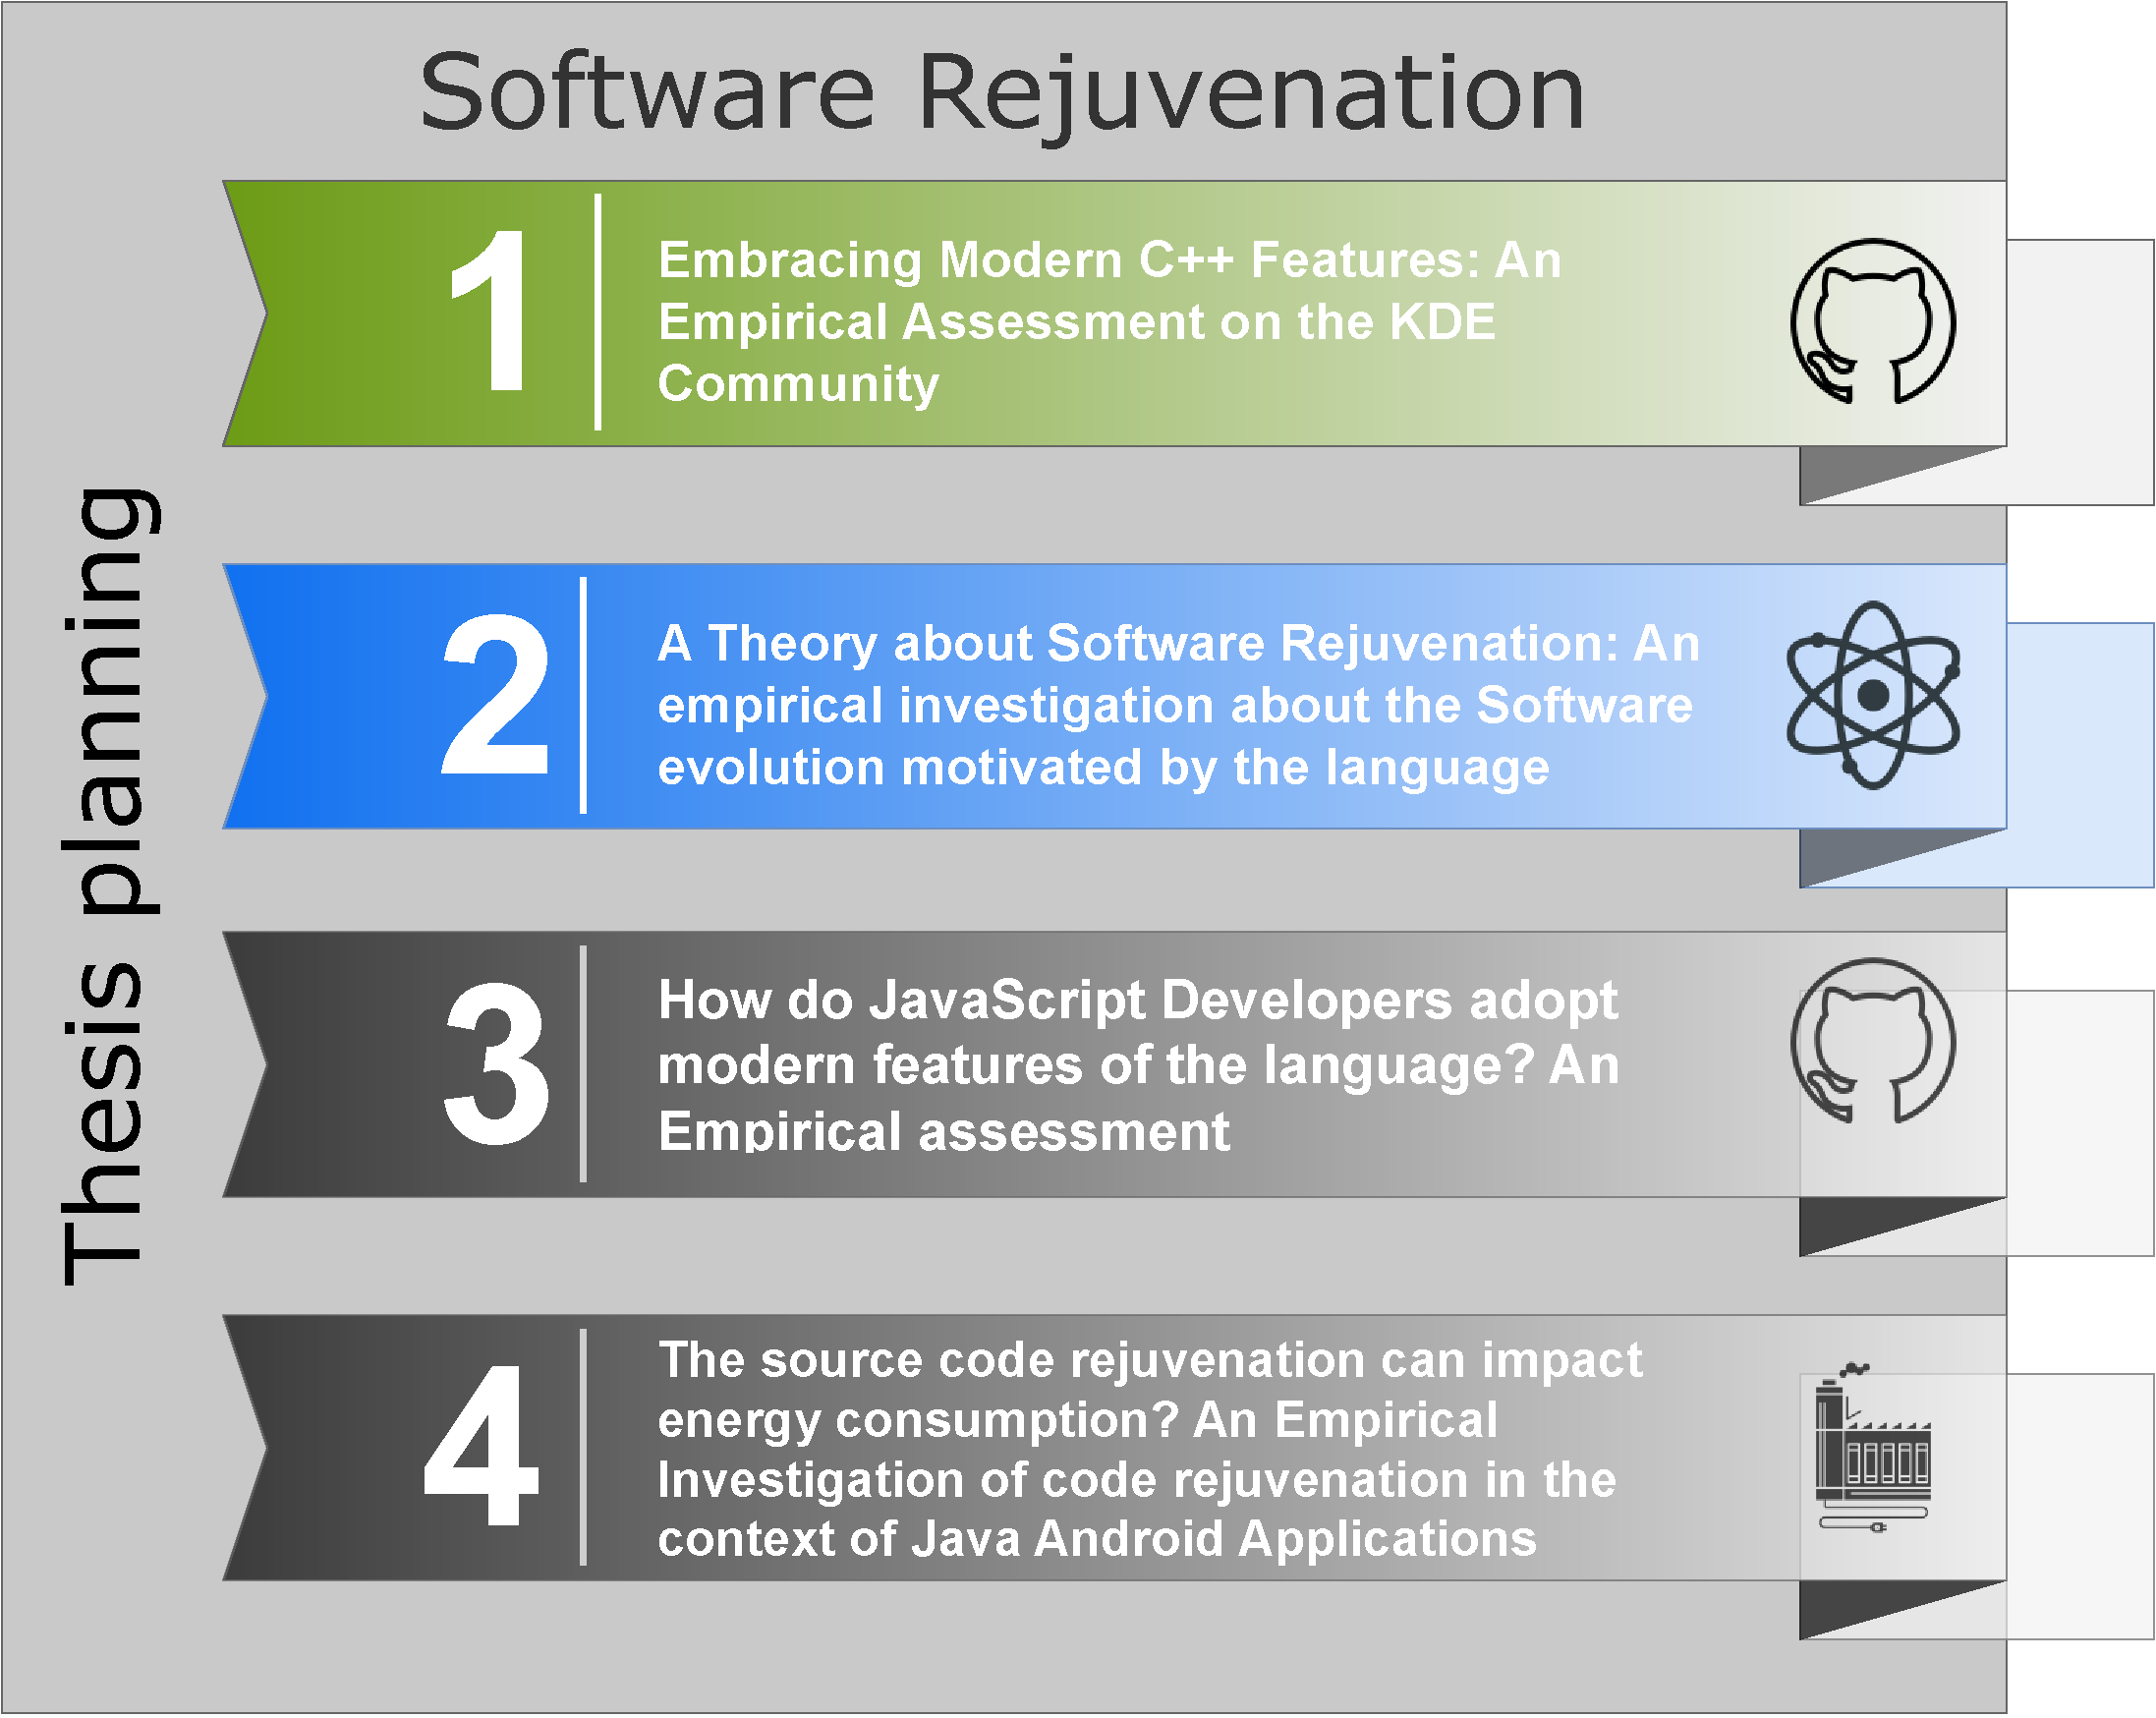
\includegraphics[width=0.7\textwidth]{images/thesis-planing.pdf}
\end{figure}
\end{frame}

%-=-=-=-=-=-=-=-=-=-=-=-=-=-=-=-=-=-=-=-=-=-=-=-=
%	FRAME: Theme Options
%-=-=-=-=-=-=-=-=-=-=-=-=-=-=-=-=-=-=-=-=-=-=-=-=

%-=-=-=-=-=-=-=-=-=-=-=-=-=-=-=-=-=-=-=-=-=-=-=-=
%
%	SECTION: COLORS
%
%-=-=-=-=-=-=-=-=-=-=-=-=-=-=-=-=-=-=-=-=-=-=-=-=
\section{Study 1: Embracing Modern C++ Features (KDE)}

%-=-=-=-=-=-=-=-=-=-=-=-=-=-=-=-=-=-=-=-=-=-=-=-=
%	TEMPLATE OF BASIC FRAME
%-=-=-=-=-=-=-=-=-=-=-=-=-=-=-=-=-=-=-=-=-=-=-=-=
\begingroup
\setbeamercolor{frametitle}{bg=\cnGreen}
\begin{frame}[c]{Research Questions}

We investigate the following research questions:
{\footnotesize
\begin{enumerate}[(RQ1)]
  \item \rqa
  \item \rqb
  \item \rqc
  \item \rqd
  \item \rqe
  \item \rqf
  \item \rqg
\end{enumerate}
}

% \begingroup
% \setbeamercolor{block title}{fg=white, bg=\cnGreen}
% \setbeamercolor{block body}{bg=\cnLightGreen}
% \begin{block}{Green Colored Blocks}
% 	Produced by using the \texttt{cblock} theme option
% \end{block}

% \begin{block}{Green Colored Blocks}
% 	Produced by using the \texttt{cblock} theme option
% \end{block}

% \begin{block}{Green Colored Blocks}
% 	Produced by using the \texttt{cblock} theme option
% \end{block}
% \endgroup

\end{frame}

%-=-=-=-=-=-=-=-=-=-=-=-=-=-=-=-=-=-=-=-=-=-=-=-=
%	FRAME:
%-=-=-=-=-=-=-=-=-=-=-=-=-=-=-=-=-=-=-=-=-=-=-=-=

\begin{frame}{Study settings and Dataset}

\begin{itemize}
    \item We realized a mixed-method study (MSR and Survey).
    \item We analyzed 272 KDE projects on GitHub (the official mirror).
    \item We found 57 commits that represent a big effort to make the code of the KDE programs more modern.
    \item We contact 11 developers that conducted rejuvenation efforts in KDE projects.
\end{itemize}

\end{frame}

%-=-=-=-=-=-=-=-=-=-=-=-=-=-=-=-=-=-=-=-=-=-=-=-=
%	FRAME:
%-=-=-=-=-=-=-=-=-=-=-=-=-=-=-=-=-=-=-=-=-=-=-=-=

\begin{frame}[c]{Fidings}

\begin{table}[ht]
  \centering
  \caption{Adoption of modern \cc features in KDE projects.}\label{tab:adoption}
  \scalebox{0.7}{
    \begin{tabular}{lrcc}
      \hline
      Feature            & Projects Adoption (\%) & Occurrences (\#) & First Occurrence \\
      \hline
      \autoDecl          & 80.51                  & 33225            & Mar-2010         \\
      \constExp          & 14.70                  & 777              & Nov-2012         \\
      \ifWithInitializer & 4.4                  & 71               & May-2020         \\
      \lambdaExp         & 63.60                  & 8918             & Mar-2010         \\
      \rangeFor          & 78.30                  & 16485            & Dec-2011         \\
      \threadDeclaration & 0.73                   & 6                & May-2018         \\
      \hline
    \end{tabular}}
\end{table}

\end{frame}

%-=-=-=-=-=-=-=-=-=-=-=-=-=-=-=-=-=-=-=-=-=-=-=-=
%	FRAME:
%-=-=-=-=-=-=-=-=-=-=-=-=-=-=-=-=-=-=-=-=-=-=-=-=

\begin{frame}{Fidings}

\begin{figure}[ht]
  \centering
  \caption{\footnotesize Distribution of \lambdaExp usage across the KDE projects in our dataset.}
  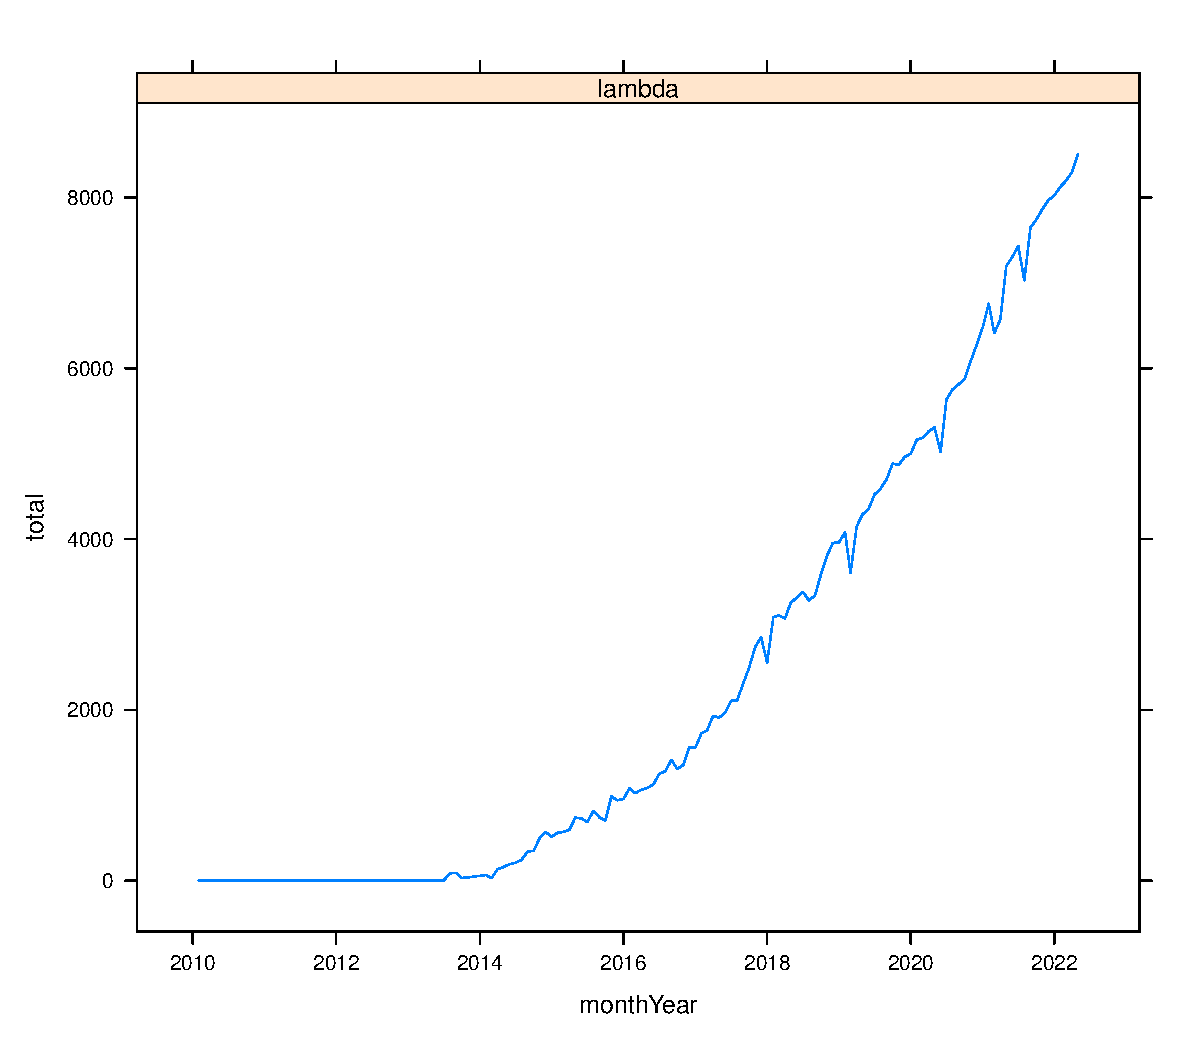
\includegraphics[width=0.7\textwidth]{images/lambda.pdf}
  \label{fig:lambda}
\end{figure}

\end{frame}

%-=-=-=-=-=-=-=-=-=-=-=-=-=-=-=-=-=-=-=-=-=-=-=-=
%	FRAME:
%-=-=-=-=-=-=-=-=-=-=-=-=-=-=-=-=-=-=-=-=-=-=-=-=

\begin{frame}{Fidings}

\begin{figure}[ht]
  \centering
  \caption{\footnotesize Distribution of \autoDecl, and \rangeFor usage across the KDE projects in our dataset.}
  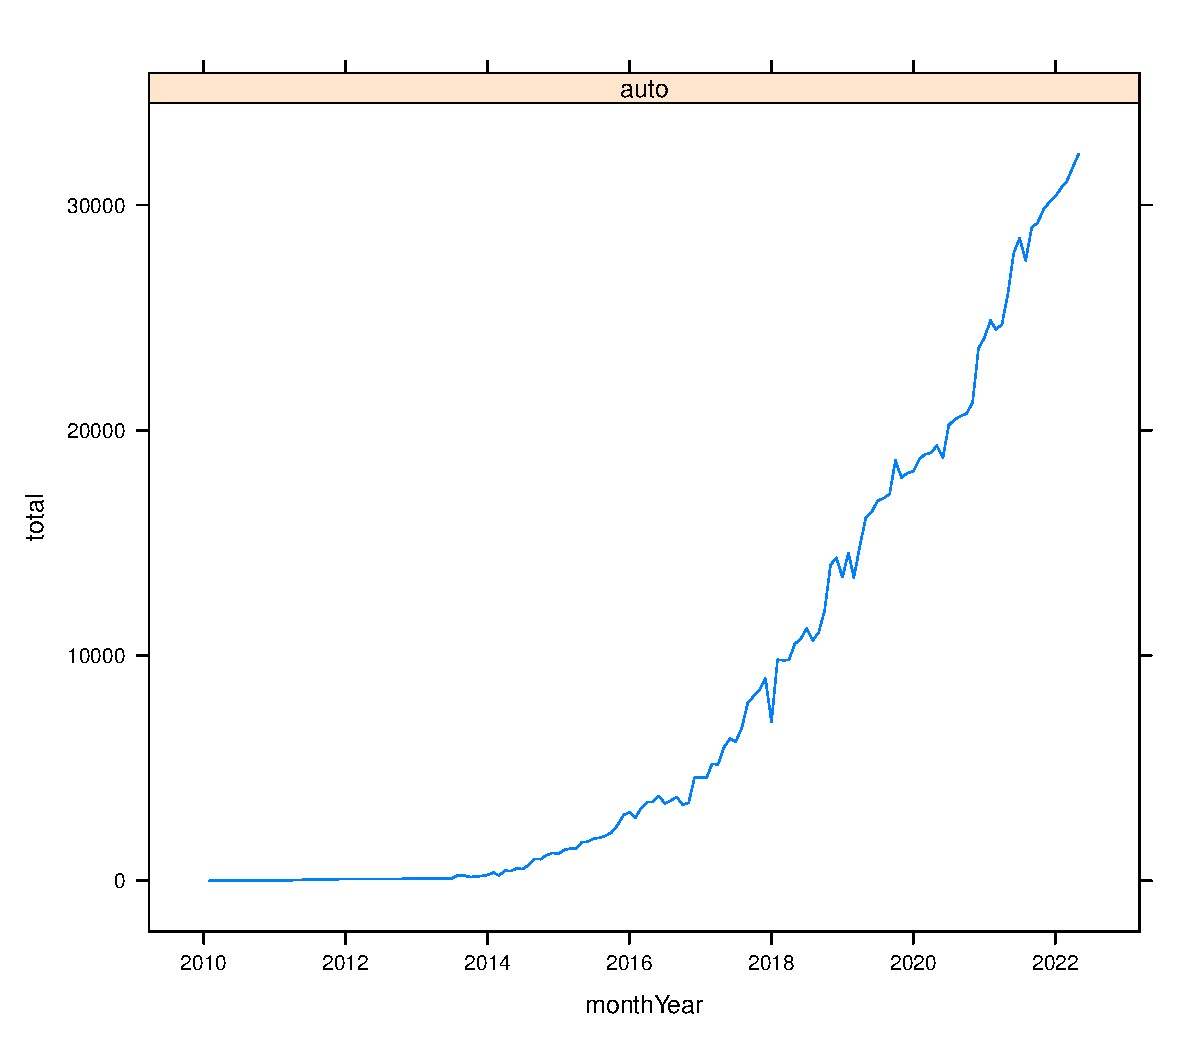
\includegraphics[width=.49\textwidth]{images/auto.pdf}\hfill
  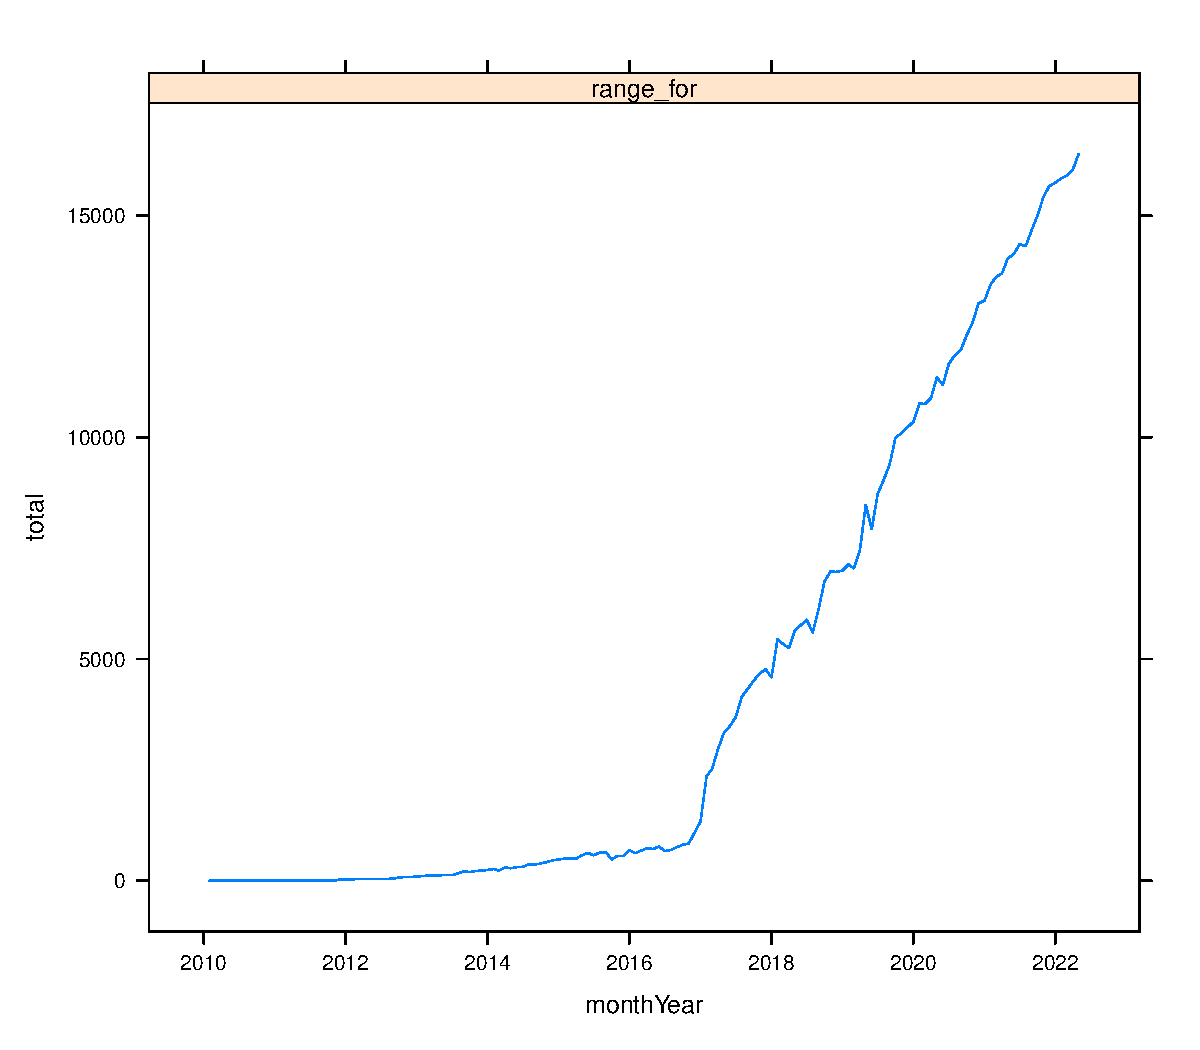
\includegraphics[width=.49\textwidth]{images/range_for.pdf}\hfill
  \label{fig:features}
\end{figure}

\end{frame}

%-=-=-=-=-=-=-=-=-=-=-=-=-=-=-=-=-=-=-=-=-=-=-=-=
%	FRAME:
%-=-=-=-=-=-=-=-=-=-=-=-=-=-=-=-=-=-=-=-=-=-=-=-=

\begin{frame}{Implications}

{\footnotesize
\begin{itemize}
\item We present a list of benefits and rejuvenation scenarios that developers can adopt in their programs. Our results show that using \lambdaExp, \autoDecl, and \rangeFor improves the readability of the code and facilitates the maintainability of the software. 

\item Our results demonstrate the use of automated tools (Clazy, Clang-tidy, KDevelop, and Clion) to help KDE developers identify rejuvenation scenarios.

\item We found evidence that external libraries have features that are good alternatives for multithreading in \cc---this motivates the KDE community not to use the new support for \cc thread available in the standard library. 

\item We present a catalog of commits that characterizes rejuvenation efforts.
\end{itemize}
}

\end{frame}
\endgroup
%-=-=-=-=-=-=-=-=-=-=-=-=-=-=-=-=-=-=-=-=-=-=-=-=
%	FRAME:
%-=-=-=-=-=-=-=-=-=-=-=-=-=-=-=-=-=-=-=-=-=-=-=-=

% \begin{frame}{Collaborators}


% \end{frame}

\section{Study 2: A Theory about Software Rejuvenation}

%-=-=-=-=-=-=-=-=-=-=-=-=-=-=-=-=-=-=-=-=-=-=-=-=
%	FRAME:
%-=-=-=-=-=-=-=-=-=-=-=-=-=-=-=-=-=-=-=-=-=-=-=-=
\begingroup
\setbeamercolor{frametitle}{bg=\cnBlue}
\begin{frame}[c]{Research Questions}

\begin{block}{What are the motivations that lead software developers to rejuvenate their software?}
{\color{white} This question aims to understand what factors, phenomena, and situations lead developers to rejuvenate their codes.}
\end{block}

\begin{block}{What are the challenges that hinder software developers from rejuvenating their software?}
{\color{white} This question aims to explain which situations and factors make it difficult or prevent developers to rejuvenate their programs.}
\end{block}

\end{frame}

%-=-=-=-=-=-=-=-=-=-=-=-=-=-=-=-=-=-=-=-=-=-=-=-=
%	FRAME:
%-=-=-=-=-=-=-=-=-=-=-=-=-=-=-=-=-=-=-=-=-=-=-=-=

\begin{frame}[c]{Grounded Theory Methodology}

\begin{figure}[H]
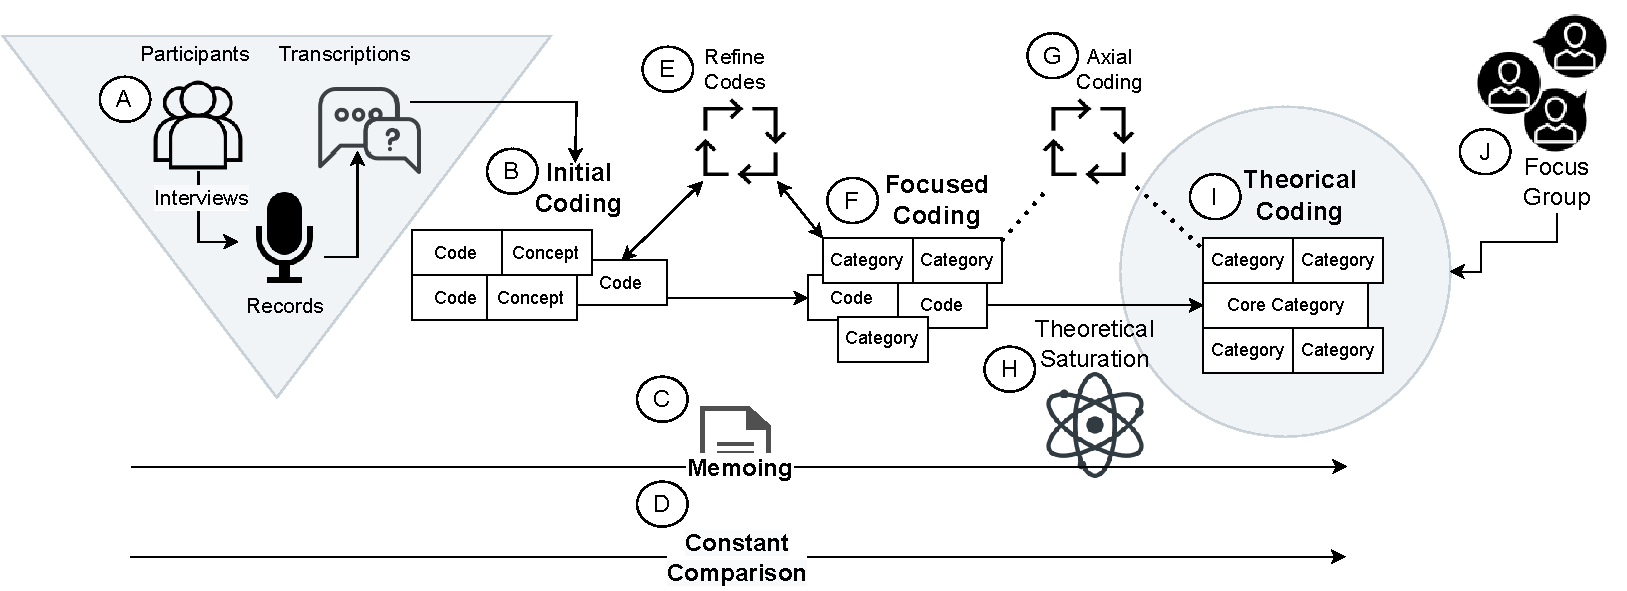
\includegraphics[width=11cm]{images/gt-overview.drawio.pdf}
\caption{Grounded Theory (Charmaz, 2016)}
\end{figure}

\end{frame}

\begin{frame}[c]{Procedures and Data Analysis}

\begin{itemize}

\item We conducted 23 interviews with experts and professional developers around the world.
\item We will conduct a focus group with expert developers in companies and organizations.

\end{itemize}

\end{frame}

\begin{frame}[c]{Conferences and Journals}

\begin{itemize}
    \item Journal of Software: Evolution and Process (JSEP) - 2023.
    \item IEEE Transactions on Software Engineering (TSE) - 2023.
    \item The International Conference on Software Maintenance and Evolution (ICSME) - 2023;
\end{itemize}

\end{frame}


% %-=-=-=-=-=-=-=-=-=-=-=-=-=-=-=-=-=-=-=-=-=-=-=-=
% %	FRAME:
% %-=-=-=-=-=-=-=-=-=-=-=-=-=-=-=-=-=-=-=-=-=-=-=-=
% \begingroup
% \setbeamercolor{background canvas}{bg=\cnDarkGrey}
% \begin{frame}[plain]

% \centering{\cDarkGrey{\Huge{THE \newline END}}}

% \end{frame}
% \endgroup

%-=-=-=-=-=-=-=-=-=-=-=-=-=-=-=-=-=-=-=-=-=-=-=-=
%	FRAME: COFFEE TIME
%-=-=-=-=-=-=-=-=-=-=-=-=-=-=-=-=-=-=-=-=-=-=-=-=
{
\usebackgroundtemplate{
\includegraphics[width=\paperwidth,height=\paperheight]{images/coffe-time.jpg}}%
\begin{frame}[plain]

% \begin{mybox}
    
% \end{mybox}

\end{frame}
}

\end{document}